\chapter{Distributions of one Variable}


\section{Characterizing a Distribution}

\subsection{Continuous Distribution Functions}

A continuous distribution function describes the \Gls{distribution} of a population, and can be represented in several equivalent ways:

\subsubsection{Probability Density Function (PDF)}\index{general}{probability density function}
The \acrfull{pdf}, or density of a continuous random variable, is a function that describes the relative likelihood for a random variable $X$ to take on a given value $x$.
In the mathematical fields of probability and statistics, a \emph{random variate x} \index{general}{random variate} is a particular outcome of a \emph{random variable X}: the random variates which are other outcomes of the same random variable might have different values.

Since the likelihood to find any given value cannot be less than zero, and since the variable has to have some value, the PDF has the following properties:

\begin{itemize}
  \item $PDF(x) \geq 0\,\forall \,x \in \mathbb{R}$
  \item $ \int\limits_{ - \infty }^\infty  {PDF(x)dx = 1} $
\end{itemize}

The PDF also defines the \emph{expected value E[x]} \index{general}{expected value} of a continuous distribution of X:

\begin{equation}\label{eq:expectedValue}
   \operatorname{E}[X] = \int_{-\infty}^\infty x f(x)\, \mathrm{d}x .
\end{equation}

\begin{figure}
  \centering
  % Requires \usepackage{graphicx}
  \includegraphics[width=0.5\textwidth]{../Images/PDF.png}\\
  \caption{Probability Density Function (PDF) of a value x. The integral over the PDF between a and b gives the likelihood of finding the value of x in that range.}\label{fig:PDF}
\end{figure}

\subsubsection{Cumulative Distribution Function (CDF)}\index{general}{cumulative distribution function}

The probability to find a value between $a$ and $b$ is given by the integral over the PDF in that range (see Fig. \ref{fig:PDF}), and the \emph{Cumulative Distribution Function} specifies which percentage of the data below any given value (Figure \ref{fig:CDF}). Together, this gives us

\begin{equation}
   \mathbb{P}(a \leq X \leq b) = \int\limits_a^b {PDF(x)dx} = CDF(b) - CDF(a)
\end{equation}


\begin{figure}[ht]
  \centering
  \includegraphics[width=0.5\textwidth]{../Images/PDF_CDF.png}\\
  \caption{\emph{Probability density function} (left) and \emph{Cumulative distribution function} (right) of a normal distribution.}\label{fig:CDF}
\end{figure}

\subsubsection{Other important presentations of Probability Densities}\index{general}{cumulative distribution function}

Figure \ref{fig:DistributionUtilities} shows a number of functions that are equivalent to the PDF, but each represent a different aspect of the probability distribution.

I will give examples which demonstrate each aspect for a normal distribution describing the size of male subjects. To obtain the respective values, one has to multiply the PDF-function etc. with the observed standard distribution, and add the mean value:

\begin{itemize}
  \item \emph{Probability density function (PDF)}: note that to obtain the probability for the variable appearing in a certain interval, you have to \emph{integrate} the PDF over that range.

      Example: What is the chance that a man is between 160 and 165 cm tall?

  \item \emph{Cumulative distribution function (CDF)}: gives the probability of obtaining a value smaller than the given value.

        Example: What is the chance that a man is less than 165 cm tall?

  \item \emph{Survival function (SF)}: 1-CDF: gives the probability of obtaining a value larger than the given value. It can also be interpreted as the proportion of data "surviving" above a certain value.

      Example: What is the chance that a man is larger than 165 cm?

  \item \emph{Percentile point function (PPF)}: the inverse of the CDF. Answers the question "Given a certain probability, what is the corresponding value for the CDF?"

    Example: Given that I am looking for a man who is smaller than 95\% of all other men, what size does the subject have to be?

  \item \emph{Inverse survival function (ISF)}: the name says it all.

      Example: Given that I am looking for a man who is larger than 95\% of all other men, what size does the subject have to be?

\end{itemize}

\begin{figure}
  \centering
  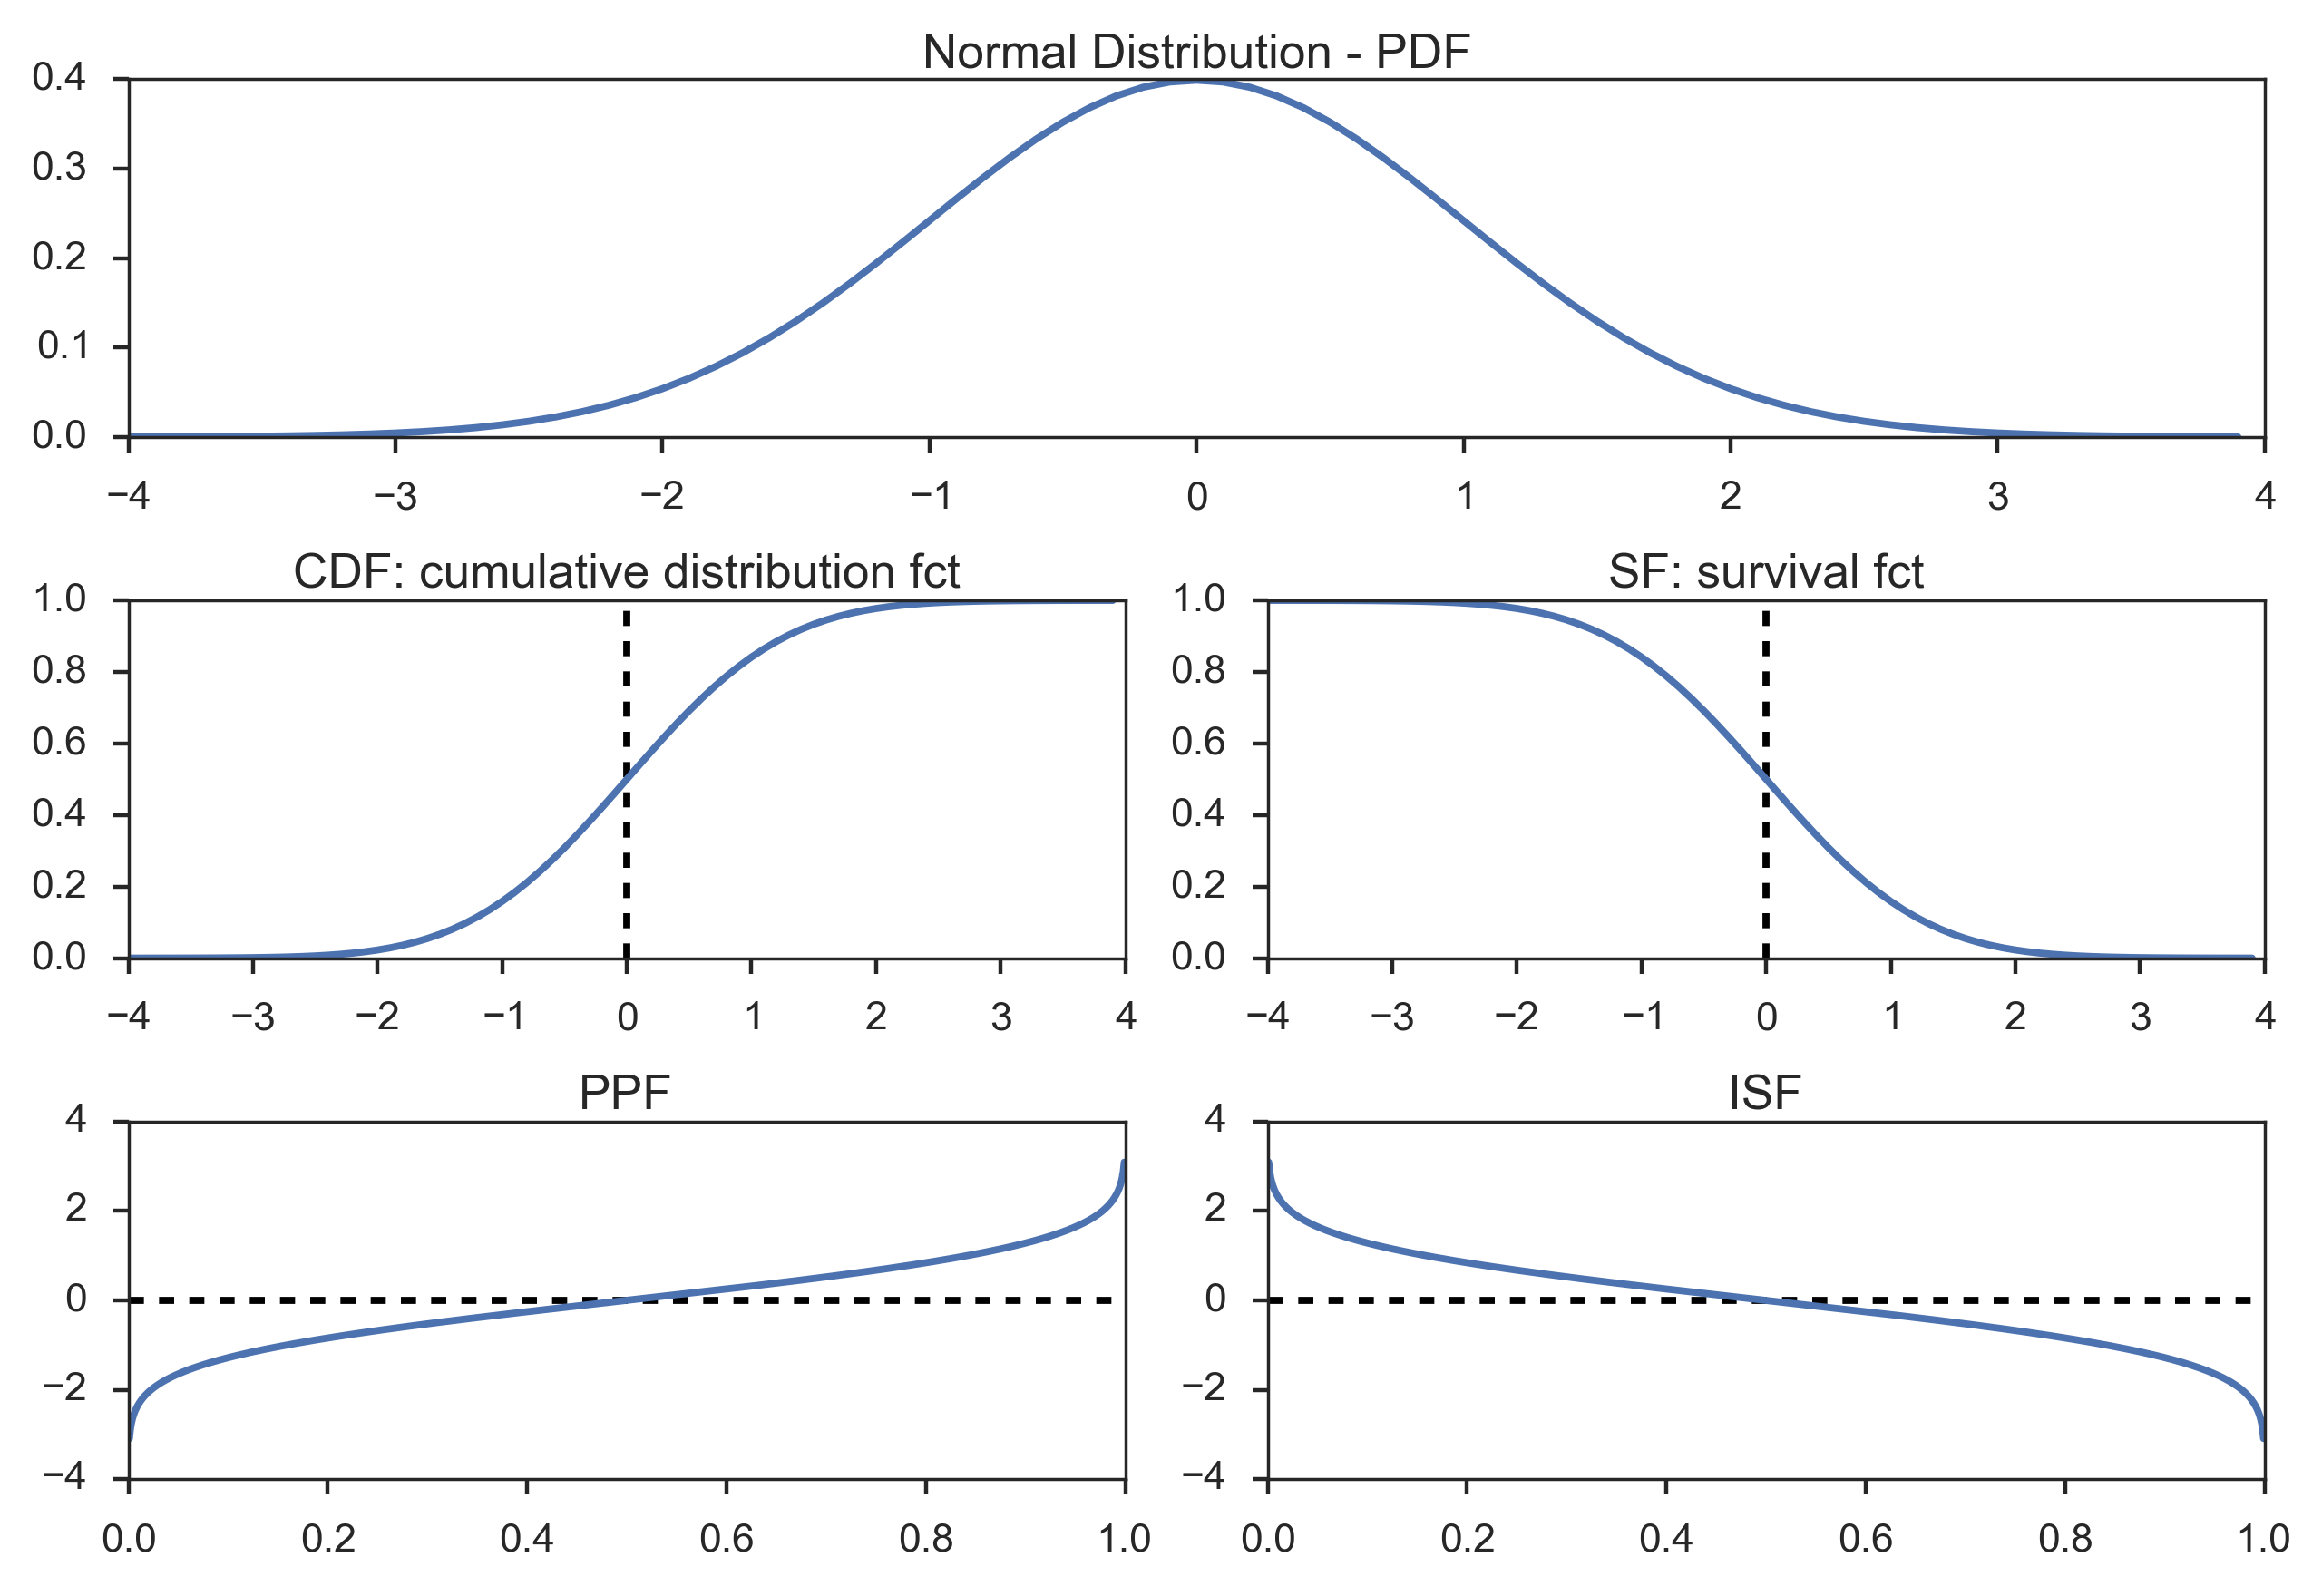
\includegraphics[width=0.95\textwidth]{../Images/DistributionFunctions.png}\\
  \caption{Utility functions for continuous distributions, here for the normal distribution.}\label{fig:DistributionUtilities}
\end{figure}

\vspace{5 mm}
\fbox{%
\begin{minipage}{15 cm}

\textbf{Note:}
In Python, the most elegant way of working with distribution function is a two-step procedure:
\begin{itemize}
  \item In the first step, you create your distribution (e.g. \textsf{nd = stats.norm()}). Note that is a \emph{distribution} (in Python parlance a "frozen distribution"\index{general}{frozen distribution}), not a function yet!
  \item In the second step, you decide which function you want to use from this distribution, and calculate the function value for the desired x-input (e.g. \textsf{y = nd.cdf(x)})
\end{itemize}

\end{minipage}}
\vspace{10 mm}

\subsection{Distribution Center}

When we have a datasample from a distribution, we can characterize the center of the distribution with different parameters:

\subsubsection{Mean} \index{general}{mean}
By default, when we talk about the \emph{mean value} we mean the \emph{arithmetic mean} $\bar{x}$:

\begin{equation}
  \bar{x} = \frac{{\sum\limits_{i = 1}^n {{x_i}} }}{n}
\end{equation}

\subsubsection{Median} \index{general}{median}
The \emph{median} is that value that comes half-way when the data are ranked in order.
In contrast to the mean, it is not affected by outlying data points.

\subsubsection{Mode} \index{general}{mode}
The \emph{mode} value is the most frequently occurring value in a distribution.

\subsubsection{Geometric Mean}\index{general}{geometric mean}
In some situations the \emph{geometric mean} can be useful to describe the location of a distribution. It is usually close to the median, and can be calculated via the arithmetic mean of the log of the values.

\subsection{Quantifying Variability}\label{sec:centiles}

\subsubsection{Range}\index{general}{range}
This one is fairly easy: it is the difference between the highest and the lowest data value.
The only thing that you have to watch out for: after you have acquired your data, you have to check for \emph{outliers}, i.e. data points with a value much higher or lower than the rest of the data. Often, such points are caused by errors in the selection of the sample or in the measurement procedure. There are a number of tests to check for outliers. One of them is to check for data which lie more than 1.5*\emph{inter-quartile-range} (IQR) above or below the first/third quartile (see below).


\subsubsection{Percentiles}\index{general}{centiles}\index{general}{percentiles}

\emph{Centiles}, also called \emph{percentile}, give the value below which a given percentage of the values occur. It corresponds to a value with a specified cumulative frequency. While you won't often hear the expression \emph{centiles}, you will frequently encounter specific centiles:

\begin{itemize}
  \item When you look for the data range which includes 95\% of the data, you have to find the $2.5^{th}$ and the $97.5^{th}$ percentile of your sample distribution.
  \item The 50th percentile is the \emph{median}.
  \item Also important are the \emph{quartiles}, i.e. the 25th and the 75th percentile. The difference between them is sometimes referred to as \emph{inter-quartile range (IQR)}\index{general}{inter-quartile-range, IQR}.
\end{itemize}

Median, upper and lower quartile are used for the data display in box plots (Fig.\ref{fig:Boxplot}).

\subsubsection{Standard Deviation and Variance}

In Fig. \ref{fig:population} I sketched out how we have to use the \emph{sample statistic} to learn about the corresponding \emph{population parameter}.
The \emph{maximum likelihood estimator of the sample variance} is given by

\begin{equation}\label{eq_variance} \index{general}{variance}
  var = \frac{{\sum\limits_{i = 1}^n {({x_i-\bar{x}})^2} }}{n}
\end{equation}

The best \emph{estimate of the population variance} is given by
However, this systematically underestimates the \emph{population variance}, and is therefore referred to as a \emph{biased estimator}\index{general}{biased estimator}.

Figure \ref{fig:mean_std} indicates that the sample variance underestimates the population variance, because the sample mean is chosen such as to minimize the variance of the data.

\begin{figure}[ht]
  \centering
  \includegraphics[width=0.5\textwidth]{../Images/mean_std.png}\\
  \caption{Gaussian distributions fitted to selections of data from the underlying distribution: While the average mean of a number of samples converges to the real mean, the sample standard deviation underestimates the standard deviation from the distribution.}\label{fig:mean_std}
\end{figure}

Division by $n-1$ corrects for this bias, and provides the best possible estimate of the population variance. The variance calculated with $n-1$ is called the \emph{sample variance}.


The \emph{standard deviation} \index{general}{standard deviation} is simply given by the square root of the variance:

\begin{equation}
  s = \sqrt{var}
\end{equation}

As mentioned in Table \ref{table:population}, in statistics it is often common to denote the population standard deviation with $\sigma$, and the sample standard deviation with $s$.

Watch out: in Python, by default the variance is calculated for "n". You have to set "ddof=1" to obtain the variance for "n-1":

\begin{lstlisting}
    In[19]: data = arange(7,14)

    In[20]: std(data, ddof=0)
    Out[20]: 2.0

    In[21]: std(data, ddof=1)
    Out[21]: 2.1602468994692865
\end{lstlisting}

\subsubsection{Standard Error} \index{general}{standard error}

The \emph{standard error} is the estimate of the \emph{standard deviation of a coefficient}. For example, in Fig. \ref{fig:sem}, we have used 100 datapoint from a normal distribution about \emph{5}. The more datapoints we have to estimate the mean value, the better our estimate. With 100 datapoints the standard deviation of our estimate, or \emph{standard error of the mean}, is 10 times smaller than the sample standard deviation.

\begin{figure}[ht]
  \centering
  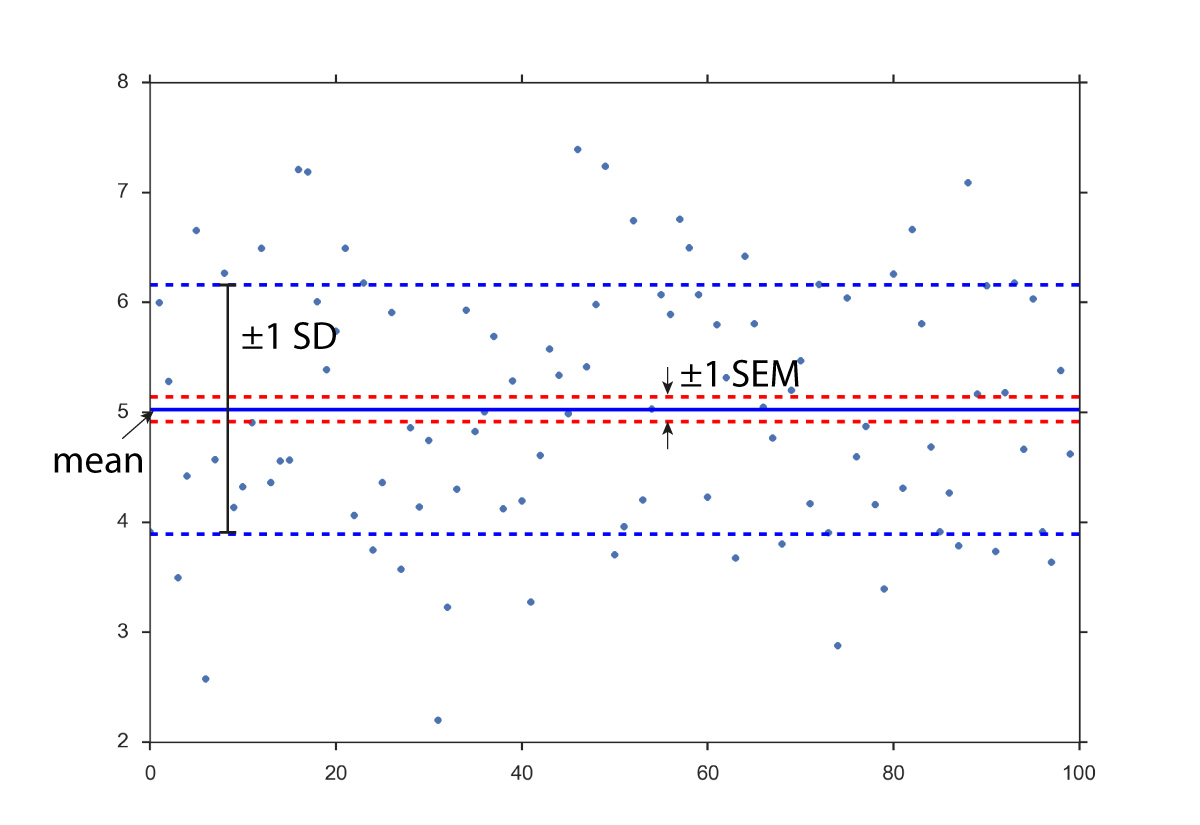
\includegraphics[width=0.66\textwidth]{../Images/standardError.jpg}\\
  \caption{100 random data points, from a normal distribution about 5. The sample mean is very close to the real mean. The standard deviation of the mean, or \emph{standard error} is 10 times smaller than the standard deviation of the samples.}
  \label{fig:sem}
\end{figure}

For normally distributed data, the \emph{sample standard error of the mean} (SE or SEM) is

\begin{equation}
  SE = \frac{s}{\sqrt{n}} = \sqrt{\frac{{\sum\limits_{i = 1}^n {({x_i-\bar{x}})^2} }}{n-1}} \cdot \frac{1}{\sqrt{n}}
\end{equation}

\subsubsection{Confidence Intervals}\index{general}{confidence interval}

 In the statistical analysis of data it has become common to state the \emph{confidence interval} of an estimated parameter. The confidence interval reports the range that contains the true value for your parameter with a likelihood of $\alpha$\%.

If the sampling distribution is symmetrical and unimodal, it will often be possible to approximate the confidence interval by

\begin{equation}\
  ci = mean \pm std * N_{ISF}(\alpha)
\end{equation}\label{eq:ci}

where $std$ is the  standard deviation, and $N_{ISF}(\alpha)$ the inverse survival function for the normal distribution. For the 95\% two-sided confidence intervals, for example, you have to set $\alpha=0.025$ and $\alpha=0.975$ .

\textbf{Note:} If you want to know the confidence interval for the mean value, you have to replace the \emph{standard deviation} by the \emph{standard error}!

\subsection{Parameters Describing the Form of a Distribution}

In \lstinline{scipy.stats}, continuous distribution functions are characterized by their \emph{location} and their \emph{scale}. Should the definition of a distribution require more than two parameters, the following parameters are called \emph{shape parameters}.  The exact meaning of each parameter can be found in the function definition.

For example, for the \emph{normal distribution}, \emph{(location/shape)} are given by \emph{(mean/standard deviation)} of the distribution. In contrast, for the \emph{uniform distribution}, \emph{location/shape} are given by the \emph{(start/end)} of the range where the distribution is different from zero.

\subsubsection{Location}\index{general}{distribution!location}

A \emph{location parameter} $x_0$  determines the "location" or shift of a distribution.

\begin{equation*}
  f_{x0}(x)=f(x-x_0)
\end{equation*}

Examples of location parameters include the mean, the median, and the mode.

\subsubsection{Scale}\index{general}{distribution!scale}

The \emph{scale parameter} describes the width of a probability distribution.  If s is large, then the distribution will be more spread out; if s is small then it will be more concentrated. If the probability density exists for all values of $s$, then the density (as a function of the scale parameter only) satisfies

\begin{equation*}
   f_s(x) = f(x/s)/s,
\end{equation*}

where f is the density of a standardized version of the density.

\subsubsection{Shape Parameters}\index{general}{shape parameters}

It is customary to refer to all of the parameters beyond \emph{location} and \emph{scale} as \emph{shape paraemters}. Thankfully, almost all of the distributions that we use in statistics have only one or two parameters. It follows that the \emph{skewness }and \emph{kurtosis} of these distribution are constants.

\begin{figure}
  \centering
  \includegraphics[width=0.66\textwidth]{../Images/Skewness.png}\\
  \caption{Left) Normal distribution, and distribution with positive skewness. Right) The (leptokurtic) Laplace distribution has an excess kurtosis of 3, and the (platykurtic) Wigner semicircle distribution an excess kurtosis of -1.}\label{fig:skewkurtosis}
\end{figure}

\subsubsection{Skewness}\index{general}{skewness}

Distributions are \emph{skewed} if they depart from symmetry (Fig. \ref{fig:skewkurtosis}, left). For example, if you have a measurement that cannot be negative, which is usually the case, then we can infer that the data have a skewed distribution if the standard deviation is more than half the mean. Such an asymmetry is referred to as \emph{positive skewness}. The opposite, negative skewness, is rare.

\subsubsection{Kurtosis}\index{general}{kurtosis}

Kurtosis is any measure of the "peakedness" of the probability distribution (Fig. \ref{fig:skewkurtosis}, right), where the normal distribution is taken as the standard refernence. Distributions with negative or positive excess kurtosis are called \emph{platykurtic} distributions or \emph{leptokurtic} distributions, respectively.

%(Lecture 5)

\section{Distribution Functions}

The variable for a standardized distribution function is often called \emph{statistic}\index{general}{statistic}. So you often find expressions like "the z-statistic" (for the normal distribution function), the "t-statistic" (for the t-distribution) or the "F-statistic" (for the F-distribution).

\subsection{Normal Distribution} \label{sec:normalDistribution}\index{general}{distributions!normal}\index{general}{normal distribution}

The \emph{Normal distribution} or \emph{Gaussian distribution} is by far the most important of all the distribution functions. This is due to the fact that the \emph{mean }values of \emph{all} distribution functions approximate a normal distribution for large enough sample numbers (see chapter \ref{sec:CentralLimitTheorem}).
Mathematically, the normal distribution is characterized by a mean value $\mu$, and a standard deviation $\sigma$:

\begin{equation}\label{eq_normal}
     f_{\mu,\sigma} (x) = \frac{1}{\sigma \sqrt{2 \pi}} e^{-( x - \mu )^2 /2 \sigma^2}
\end{equation}
where $ - \infty < x < \infty $, and $f_{\mu,\sigma}$ is the \emph{probability density function (PDF)} \index{general}{probability density function}.

\begin{figure}
  \centering
  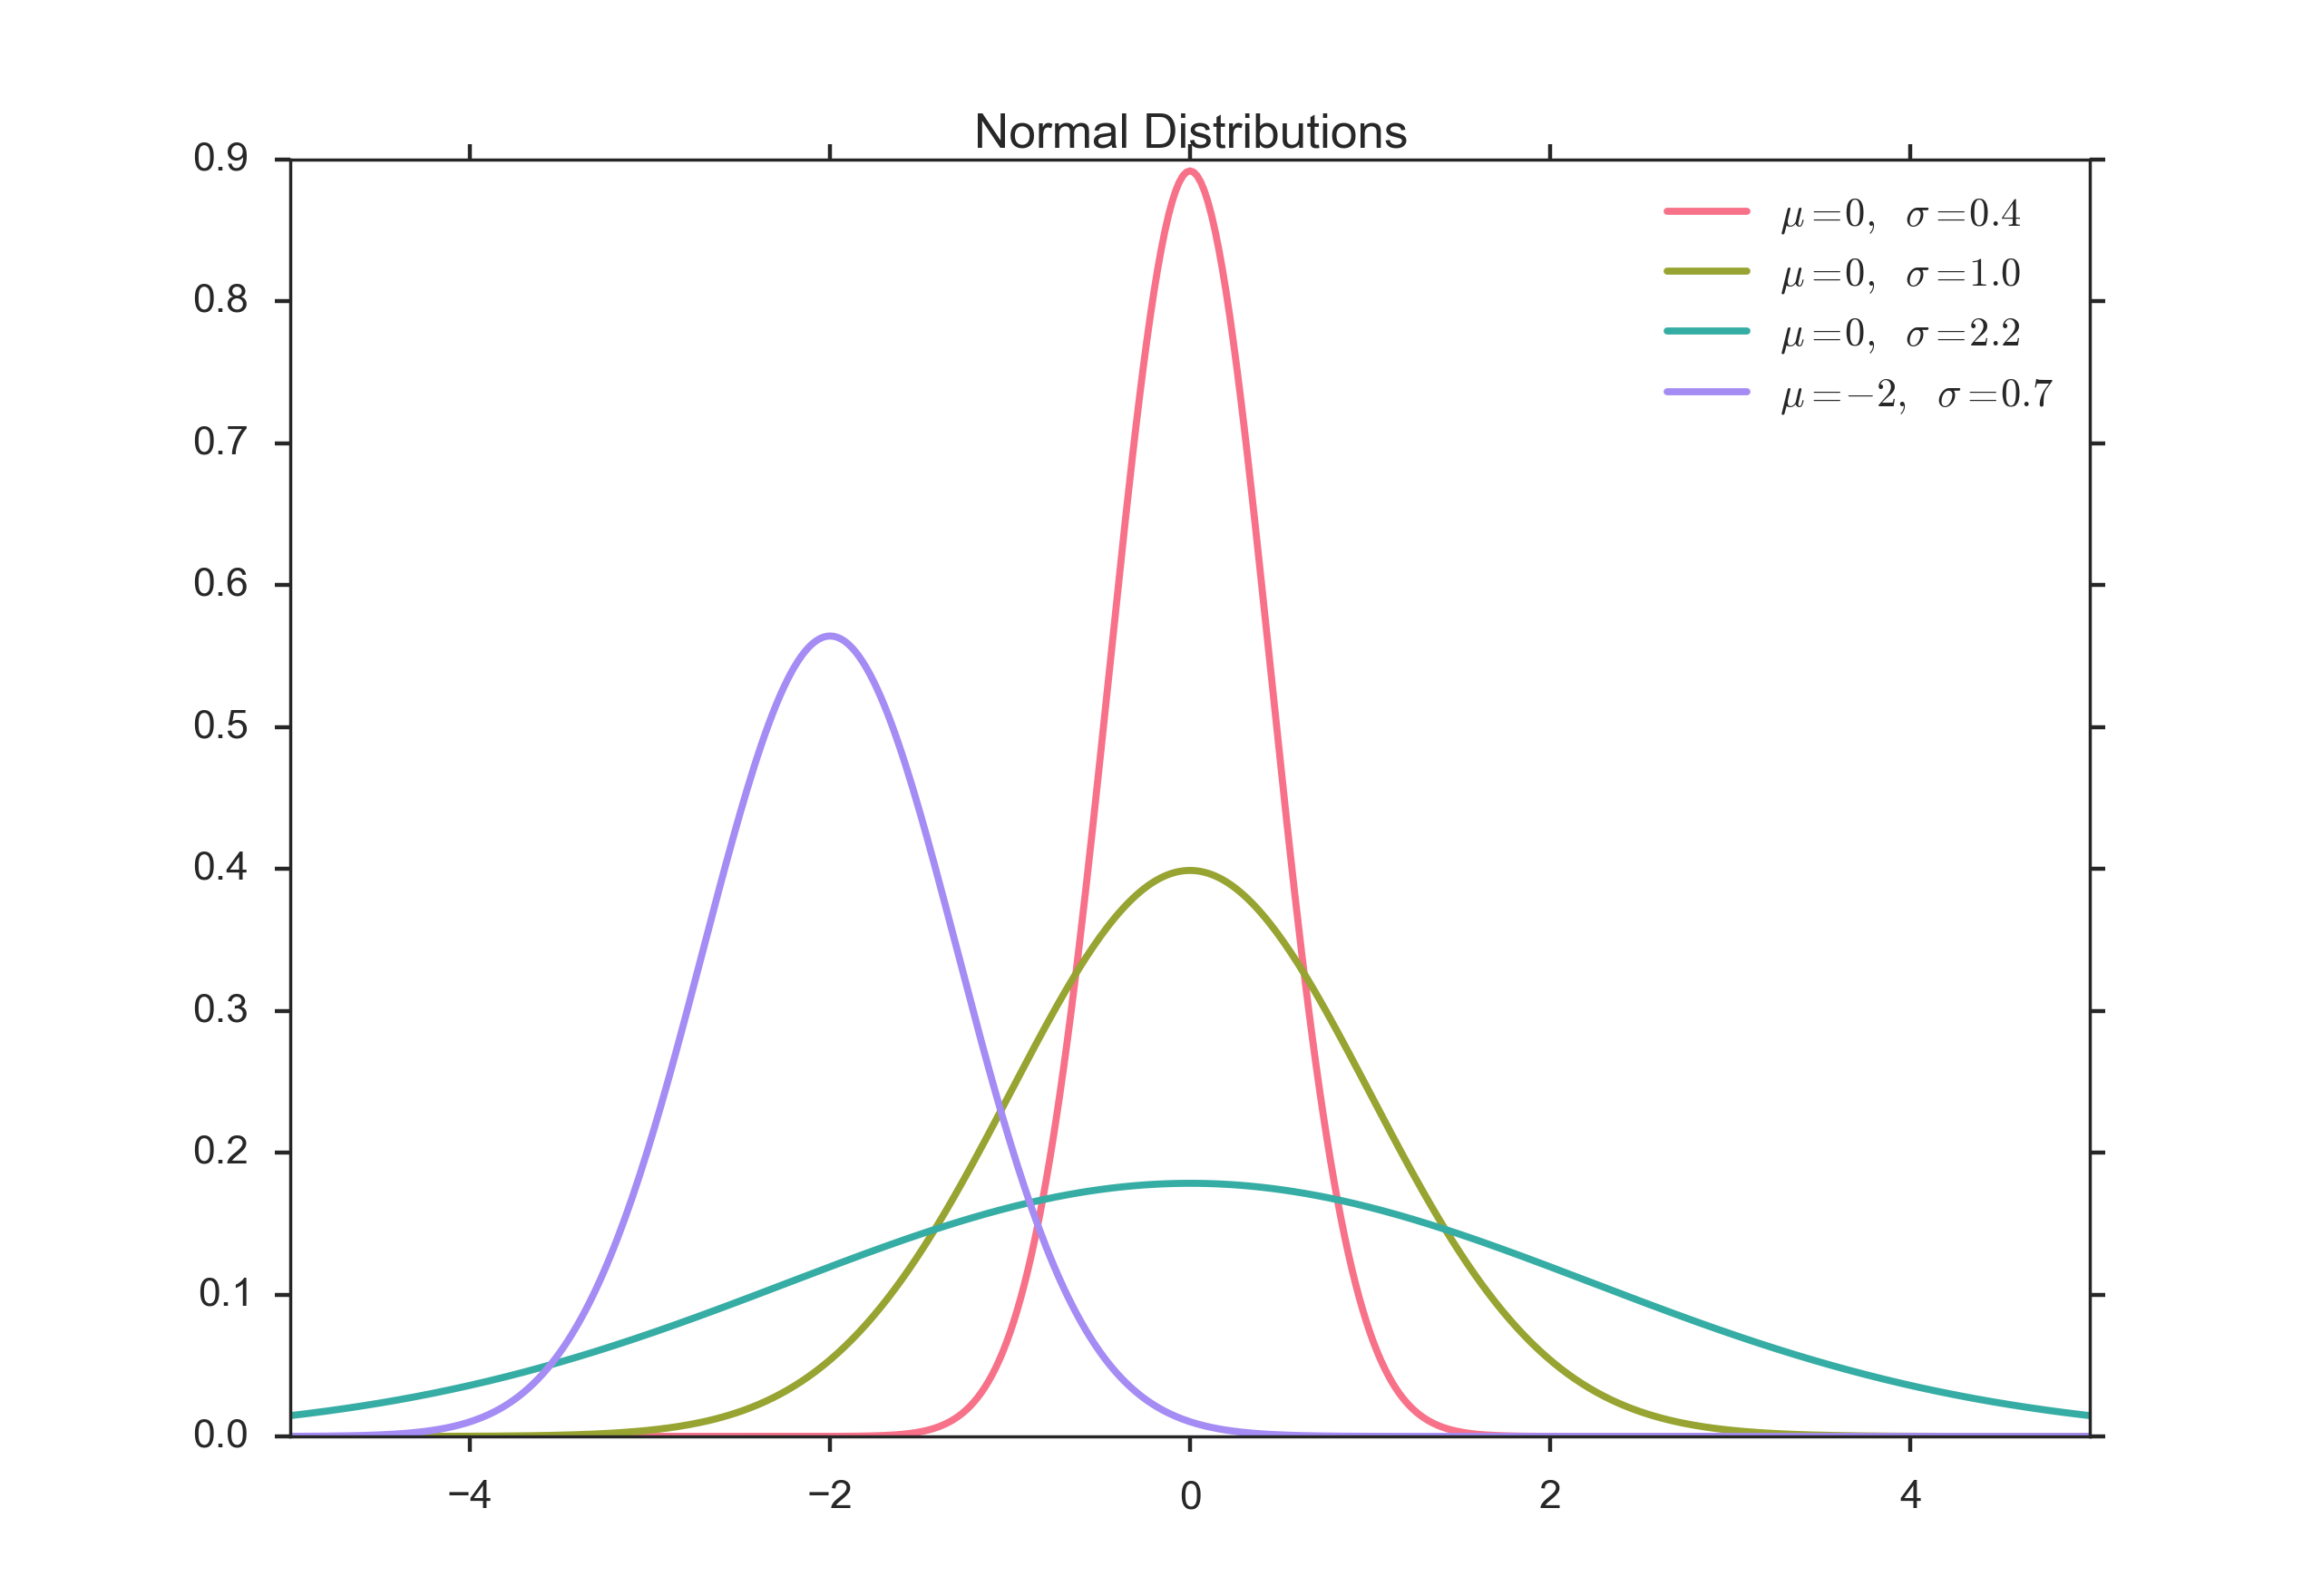
\includegraphics[width=0.75\textwidth]{../Images/Normal_Distribution_PDF.png}\\
  \caption{Normal Distribution}\label{fig:normal}
\end{figure}

For smaller sample numbers, the sample distribution can show quite a bit of variability. For example, look at 25 distributions generated by sampling 100 numbers from a normal distribution (Fig. \ref{fig:MultipleNormal})

\begin{figure}
  \centering
  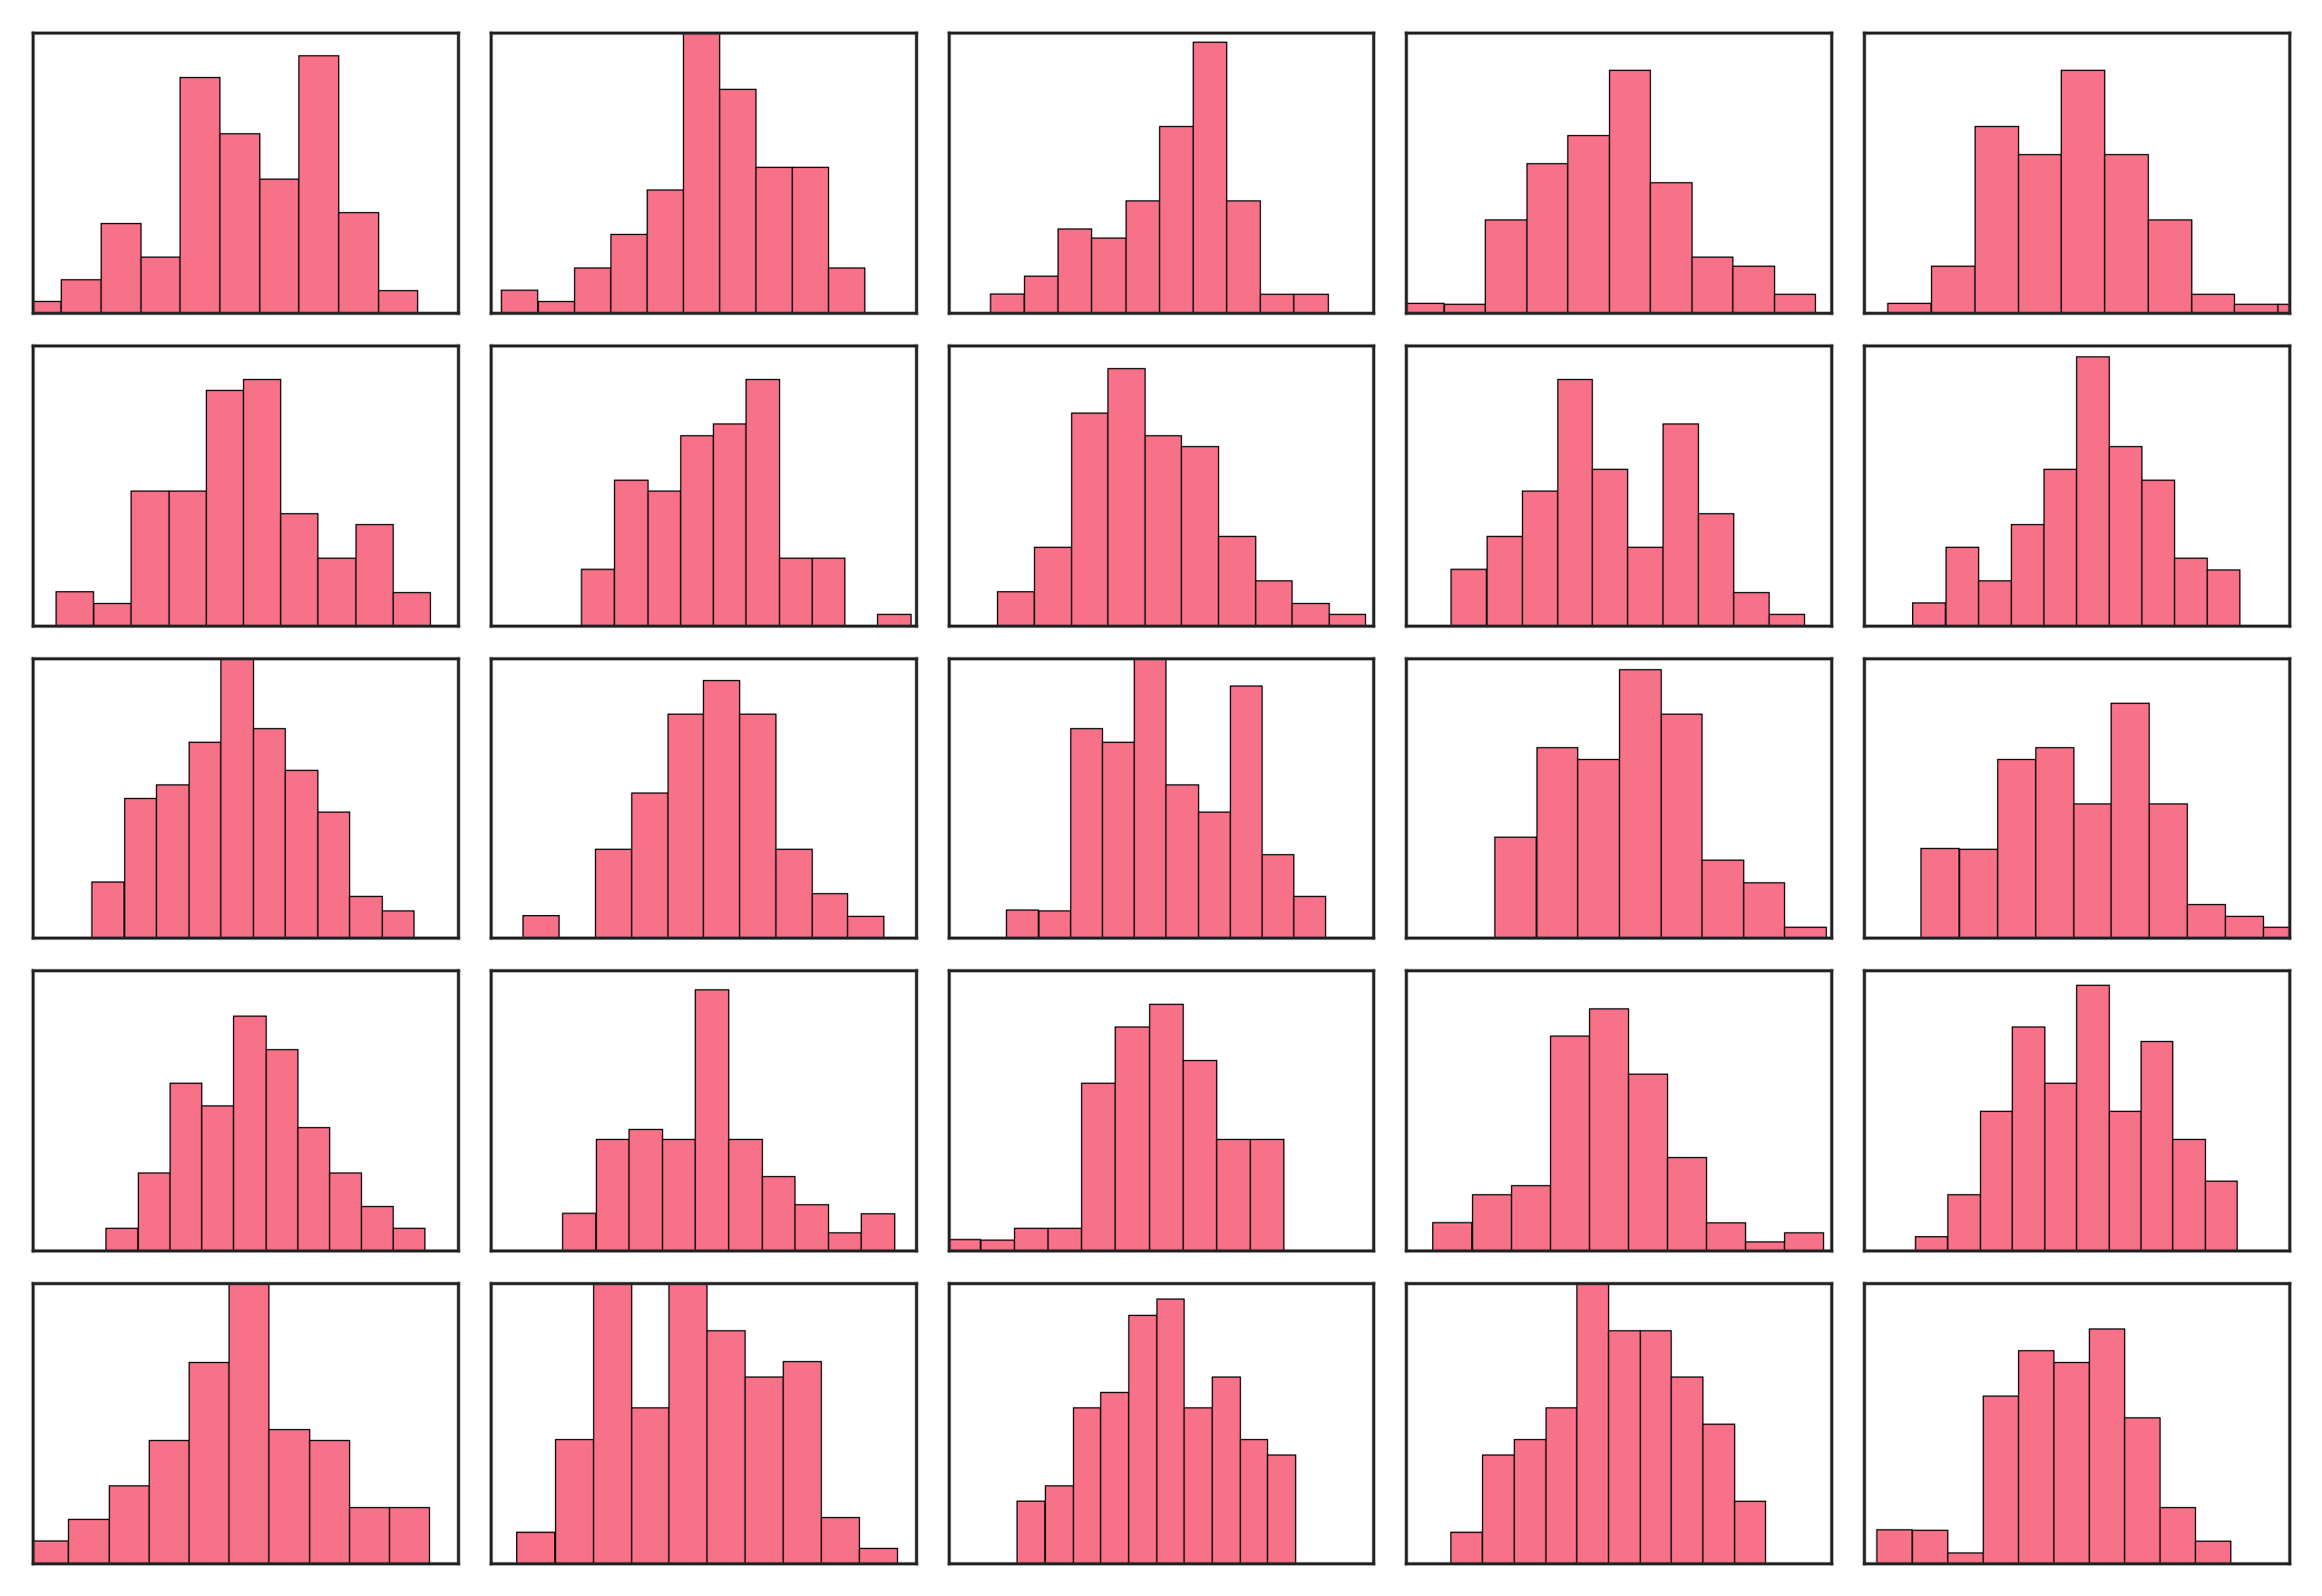
\includegraphics[width=0.75\textwidth]{../Images/Normal_MultHist.png}\\
  \caption{25 randomly generated normal distributions of 100 points.}\label{fig:MultipleNormal}
\end{figure}

The normal distribution with parameters $\mu$ and $\sigma$ is denoted as {$N(\mu,\sigma)$}. If the \emph{random variate (rv)} {\itshape X} is normally distributed with expectation $\mu$ and standard deviation $\sigma$, one denotes: {$\,X \sim N(\mu,\sigma)$} or $\,X \in N(\mu,\sigma)$.

\begin{figure}
  \centering
  % Requires \usepackage{graphicx}
  \includegraphics[width=0.8\textwidth]{../Images/area_SDs.png}\\
  \caption{Area under +/1 1, 2, and 3 standard deviations of a normal distribution.}\label{fig:area_SDs}
\end{figure}

\begin{table}
  \centering
  \begin{tabular}{c c c}
    \hline
     & \multicolumn{2}{ c } {Probability of being} \\
    Range & within range & outside range \\
    \hline
    % after \\: \hline or \cline{col1-col2} \cline{col3-col4} ...
    mean $\pm$ 1SD & 0.683 & .317 \\
    mean $\pm$ 2SD & 0.954 & 0.046 \\
    mean $\pm$ 3SD & 0.9973 & 0.0027 \\
    \hline
  \end{tabular}
  \caption{Tails of a normal distribution.}
\end{table}

\vspace{5 mm}

\PyImg "distributionNormal.py" (p \pageref{py:distributionNormal}) shows simple manipulations of normal distribution functions.
\index{python}{distributionNormal}

\begin{lstlisting}
  In [33]:  from scipy import stats
  In [34]:  mu = -2
  In [35]:  sigma = 0.7
  In [36]:  myDistribution = stats.norm(mu, sigma)
  In [37]:  significanceLevel = 0.05
  In [38]:  myDistribution.ppf([significanceLevel/2, 1-significanceLevel/2])
  Out[38]:  array([-3.38590382, -0.61409618]
\end{lstlisting}
\emph{Example of how to calculate the interval of the PDF containing 95\% of the data, for the blue curve in Figure \ref{fig:normal}}

\subsubsection{Sum of Normal Distributions}\index{general}{normal distribution!sum of}

An important property of normal distributions is that the sum (or difference) of two normal distributions is also normally distributed. i.e., if

\begin{eqnarray*}
    X &\sim& N(\mu_X, \sigma_X^2) \\
    Y &\sim& N(\mu_Y, \sigma_Y^2) \\
    Z &=& X + Y,
\end{eqnarray*}

then

\begin{equation}\label{eq:sumOfGaussians}
    Z \sim N(\mu_X + \mu_Y, \sigma_X^2 + \sigma_Y^2).
\end{equation}

\subsubsection{Examples of Normal Distributions}\index{general}{normal distribution!examples}

\begin{itemize}
    \item If the average man is 175 cm tall with a standard deviation of 6 cm, what is the probability that a man found at random will be 183 cm tall?
    \item If cans are assumed to have a standard deviation of 4 grams, what does the average weight need to be in order to ensure that the 99\% of all cans have a weight of at least 250 grams?
   \item If the average man is 175 cm tall with a standard deviation of 6 cm and the average woman is 168 cm tall with a standard deviation of 3 cm, what is the probability that a randomly selected man will be shorter than the randomly selected woman?
\end{itemize}

\subsection{Central Limit Theorem}\label{sec:CentralLimitTheorem}\index{general}{central limit theorem}
The central limit theorem states that for identically distributed independent random variables (also referred to as \emph{random variates})\index{general}{variate}, the mean of a sufficiently large number of these variables will be approximately normally distributed. Or in other words, the sampling distribution of the mean tends toward normality, regardless of the distribution.
\ref{fig:CentralLimitTheorem} shows that averaging over 10 uniformly distributed data already produces a smooth, almost Gaussian distribution.

\begin{figure}
  \centering
  % Requires \usepackage{graphicx}
  \includegraphics[width=0.7\textwidth]{../Images/CentralLimitTheorem.png}\\
  \caption{Demonstration of the "Central Limit Theorem": Left) Histogram of random data between 0 and 1. Center) Histogram of average over two datapoints.) Right) Histogram of average over 10 datapoints.}\label{fig:CentralLimitTheorem}
\end{figure}

\PyImg "centralLimitTheorem.py" (p \pageref{py:centralLimitTheorem}) demonstrates that already averaging over 10 uniformly distributed datapoints produces an almost Gaussian distribution.
\index{python}{distributionDiscrete}

\subsection{Application Example}

To illustrate the ideas behind the use of distribution functions, let us go step-by-step through the analysis of the following problem:

The average weight of a newborn child in the US is 3.5 kg, with a standard deviation of 0.76 kg. If we want to check all children that are \emph{significantly different} from the typical baby, what should we do with a child that is born with a weight of 2.6 kg?

\begin{itemize}
  \item Find the distribution that characterizes healthy babies ($\mu=3.5, \sigma=0.76$).
  \item Calculate the CDF at the interesting value (\emph{CDF(2.6 kg) = 0.118}).
  \item Interpret the result -see Fig. \ref{fig:pdf_checkValue} (\emph{"If the baby is healthy, the chance that its weight deviates by at least the observed value from the mean is 2*11.8\% = 23.6\% - This is not significant"}).
\end{itemize}

\begin{figure}
  \centering
  \includegraphics[width=0.75\textwidth]{../Images/pdf_checkValue.png}\\
  \caption{The chance that a healthy baby weighs 2.6 kg or less is 11.8\% (darker blue area). The chance that the difference from the mean is that much is twice that much, as the lighter blue area must be added.}\label{fig:pdf_checkValue}
\end{figure}

\subsection{Other Continuous Distributions}\label{sec:ContinuousDistributions} \index{general}{distributions!continuous}

The distributions you will encounter most frequently are:

\begin{itemize}
  \item \textbf{Normal distribution} - the "ideal" continuous probability distribution
  \item \textbf{t-distribution} - for sample distributions (What you will probably use most often.)
  \item \textbf{$\chi$-square distribution} - for describing  variability
  \item \textbf{F-distribution} - for comparing variability
\end{itemize}

In the following, we will describe these distributions in more detail. Other distributions you should have heard about will be mentioned briefly:

\begin{itemize}
  \item \textbf{Lognormal distribution} - a normal distribution, plotted on an exponential scale. Often used to convert a strongly skewed distribution into a normal one.
  \item \textbf{Weibull distribution} - mainly used for reliability or survival data.
  \item \textbf{Exponential distribution} - exponential curves
  \item \textbf{uniform distribution} - when everything is equally likely.
\end{itemize}

\subsubsection{t Distribution}\index{general}{distributions!t-distribution}

In 1908 W.S. Gosset, who worked for the Guinnes brewery in Dublin, was interested in the problems of small samples, for example the chemical properties of barley where sample sizes might be as low as 3. Since in these measurements the true variance of the mean was unknown, it must be approximated by the sample standard error of the mean. And the ratio between the sample mean and the standard error had a distribution that was unknown till Gosset, under the  pseudonym "Student", solved that problem.

The corresponding distribution is the \emph{t-distribution}, and converges for larger values towards the normal distribution (Fig. \ref{fig:t}).

Since in most cases the population mean and its variance are unknown, one typically works with the t-distribution when analyzing sample data.

If $\bar{x}$ is the sample mean, and $s$ the sample standard deviation, then

\begin{equation}
  t = \frac{\bar{x}-\mu}{s/ \sqrt{n}}
\end{equation}\label{eq:Tdistribution}

A very frequent application of the t-distribution is in the calculation of confidence intervals for the mean. The \emph{width }of the 95%-confidence interval, i.e. the interval that contains the true mean with a chance of 95%, is the same width about the population mean that contains 95% of the sample means (Eq. \ref{eq:ci_t}):

\begin{equation}
  ci = mean \pm std * t_{df,\alpha}
\end{equation}\label{eq:ci_t}

\begin{lstlisting}
  In [27]: n = 20
  In [28]: df = n-1
  In [29]: alpha = 0.05
  In [30]: stats.t(df).ppf(1-alpha/2)
  Out[30]: 2.093

  In [31]: stats.norm.ppf(1-alpha/2)
  Out[31]: 1.960
\end{lstlisting}

\emph{Calculating the t-values for confidence intervals, for n = 20 and $\alpha=0.05$. For comparison, I also calculate the corresponding value from the normal distribution.}

In Python, the 95\% confidence interval for the mean can be obtained with a one-liner:

\begin{lstlisting}
    alpha = 0.95
    df = len(data)-1
    ci = stats.t.interval(alpha, df, loc=mean(data), scale=stats.sem(data))
\end{lstlisting}

\begin{figure}
  \centering
  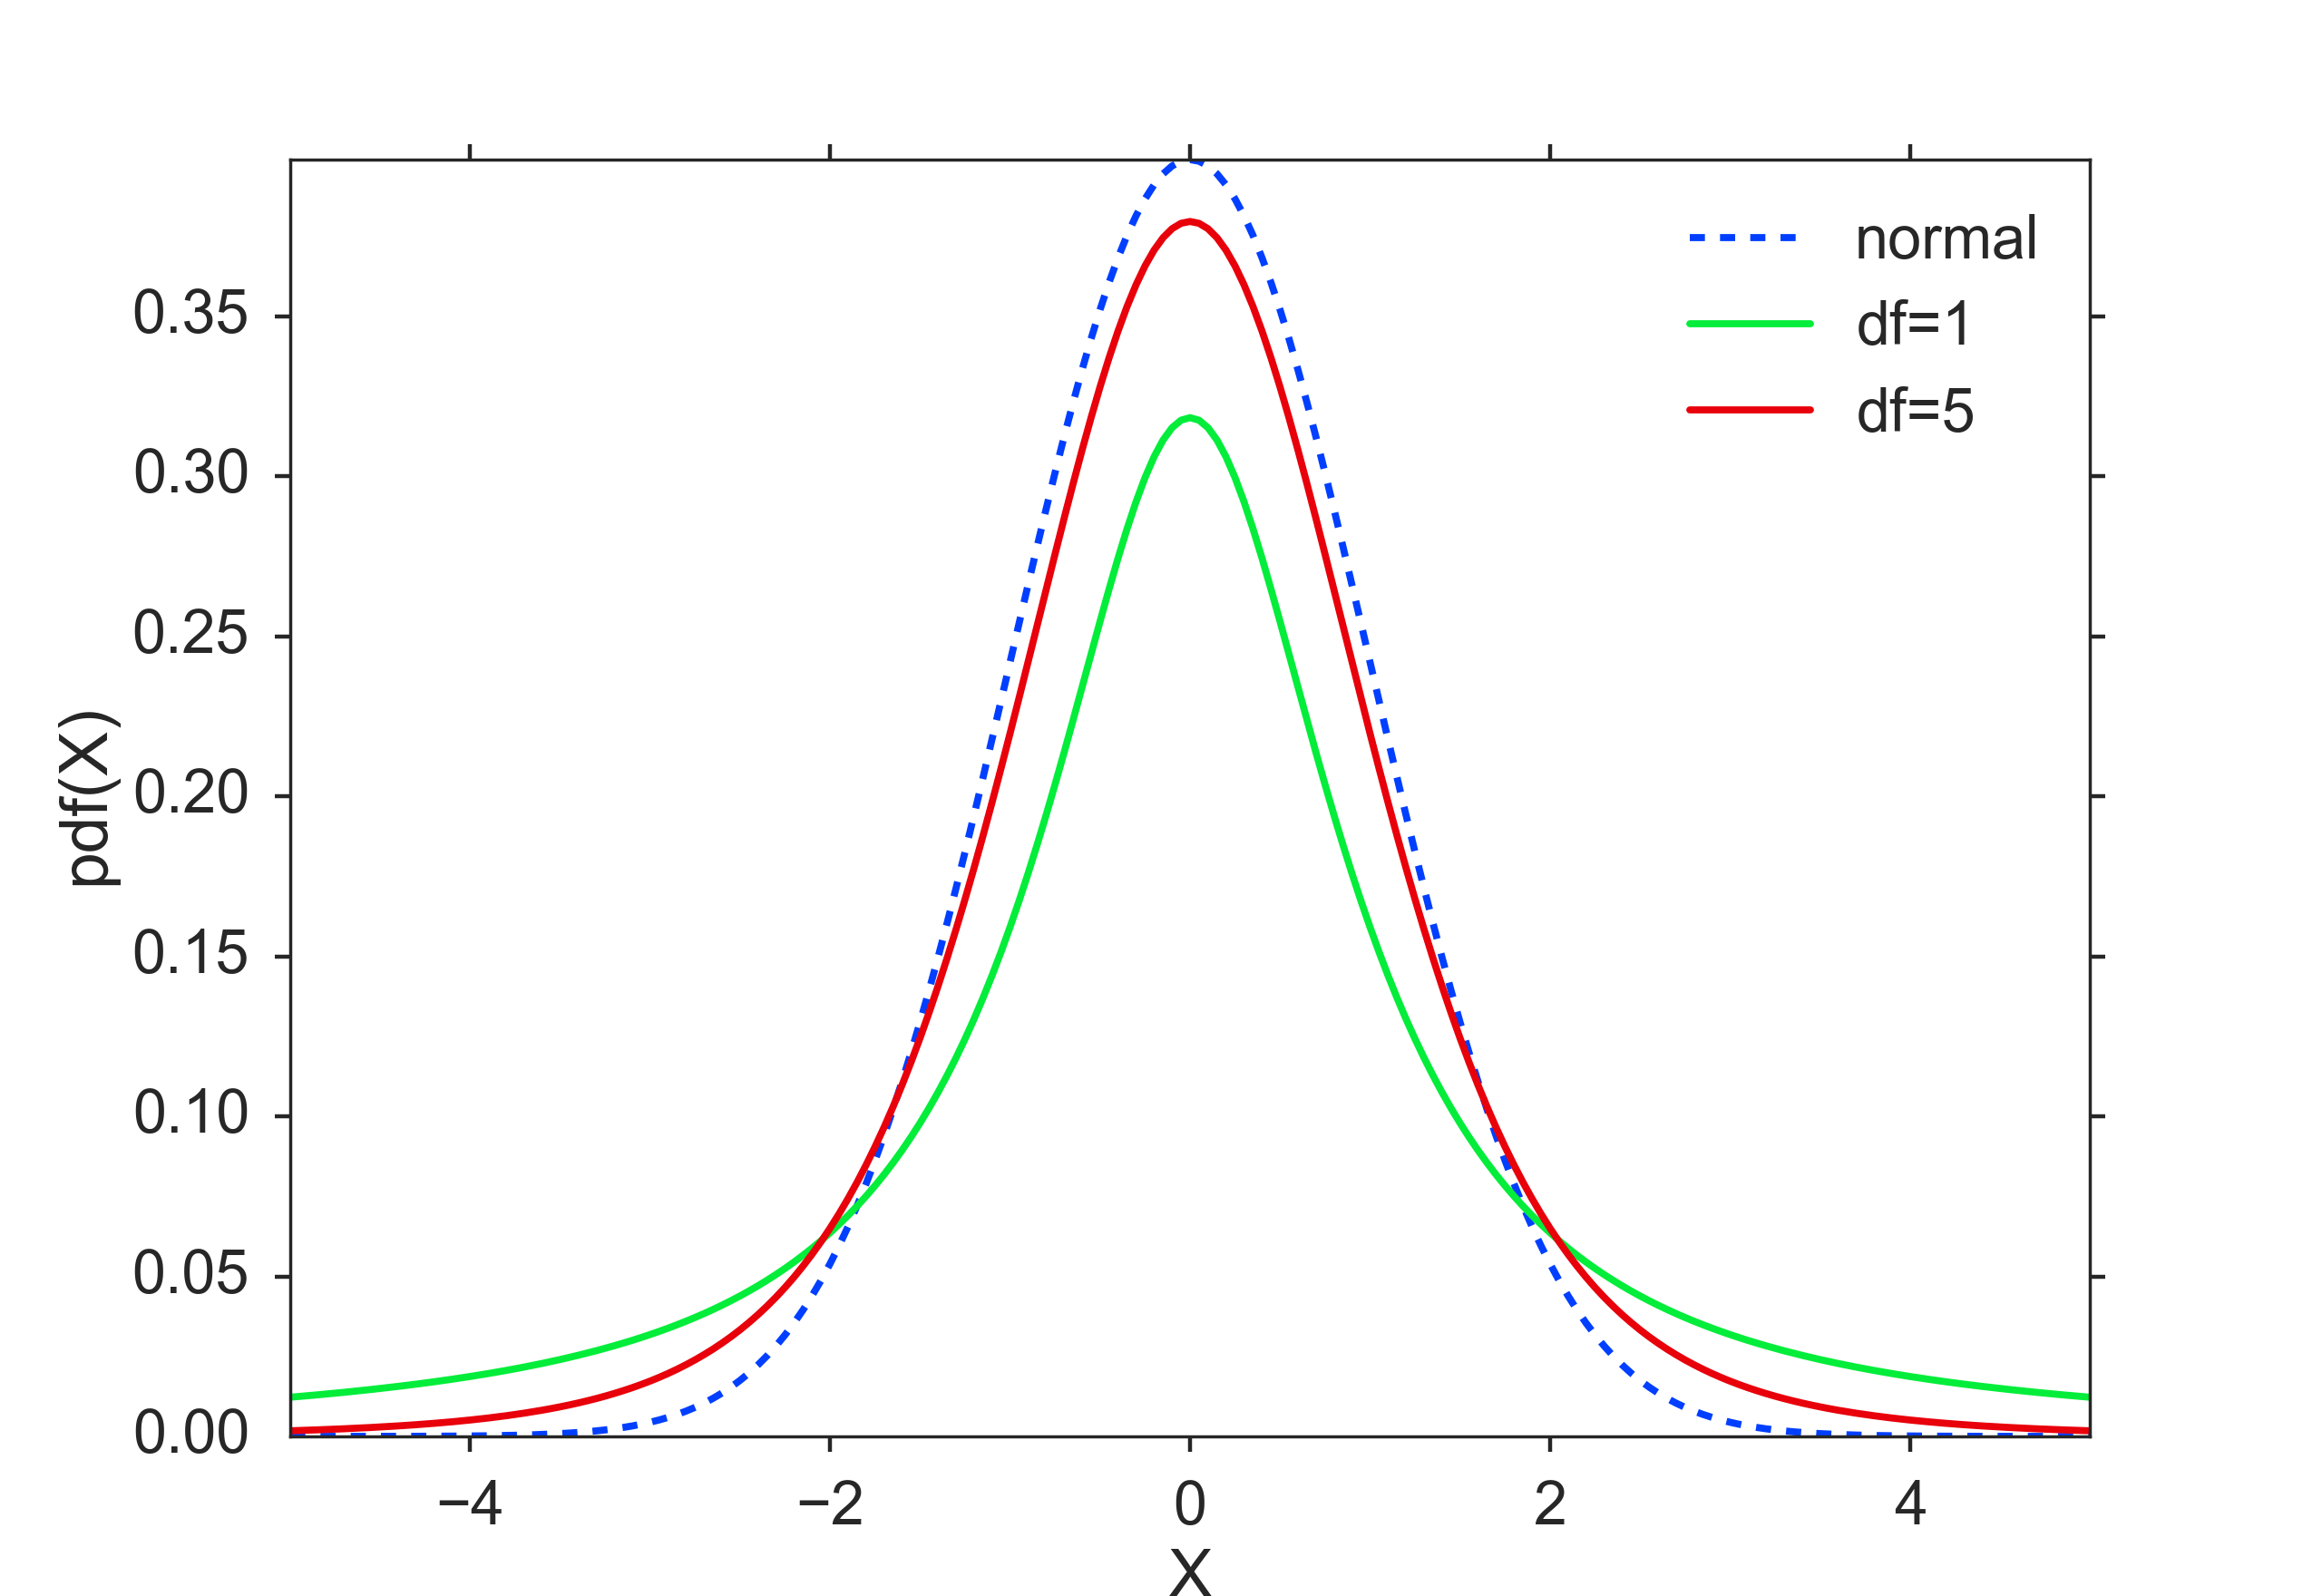
\includegraphics[width=0.5\textwidth]{../Images/dist_t.png}\\
  \caption{t Distribution}\label{fig:t}
\end{figure}

Since the t-distribution has longer tails than the normal distribution, it is much less affected by extreme cases (see Figure \ref{fig:ttest_stability}).

\begin{figure}
  \centering
  \includegraphics[width=0.75\textwidth]{../Images/ttest_stability.png}\\
  \caption{The t-distribution is much more robust against outliers than the normal distribution.}\label{fig:ttest_stability}
\end{figure}


\subsubsection{Chi-square Distribution}\index{general}{distributions!chi square}

The \emph{Chi-square distribution} is related to normal distribution in a simple way: If a random variable $X$ has a normal distribution ($X \in N(0,1)$), then $X^2$ has a chi-square distribution, with one degree of freedom ($X^2 \in \chi_{1}^2$). The \emph{sum squares }of $n$ independent and standard normal random variables has a chi-square distribution with $n$ degrees of freedom (Fig. \ref{fig:chi2}):

\begin{equation}
    \sum\limits_{i = 1}^n {X_i^2} \in \chi_{n}^2
\end{equation}


\begin{figure}
  \centering
  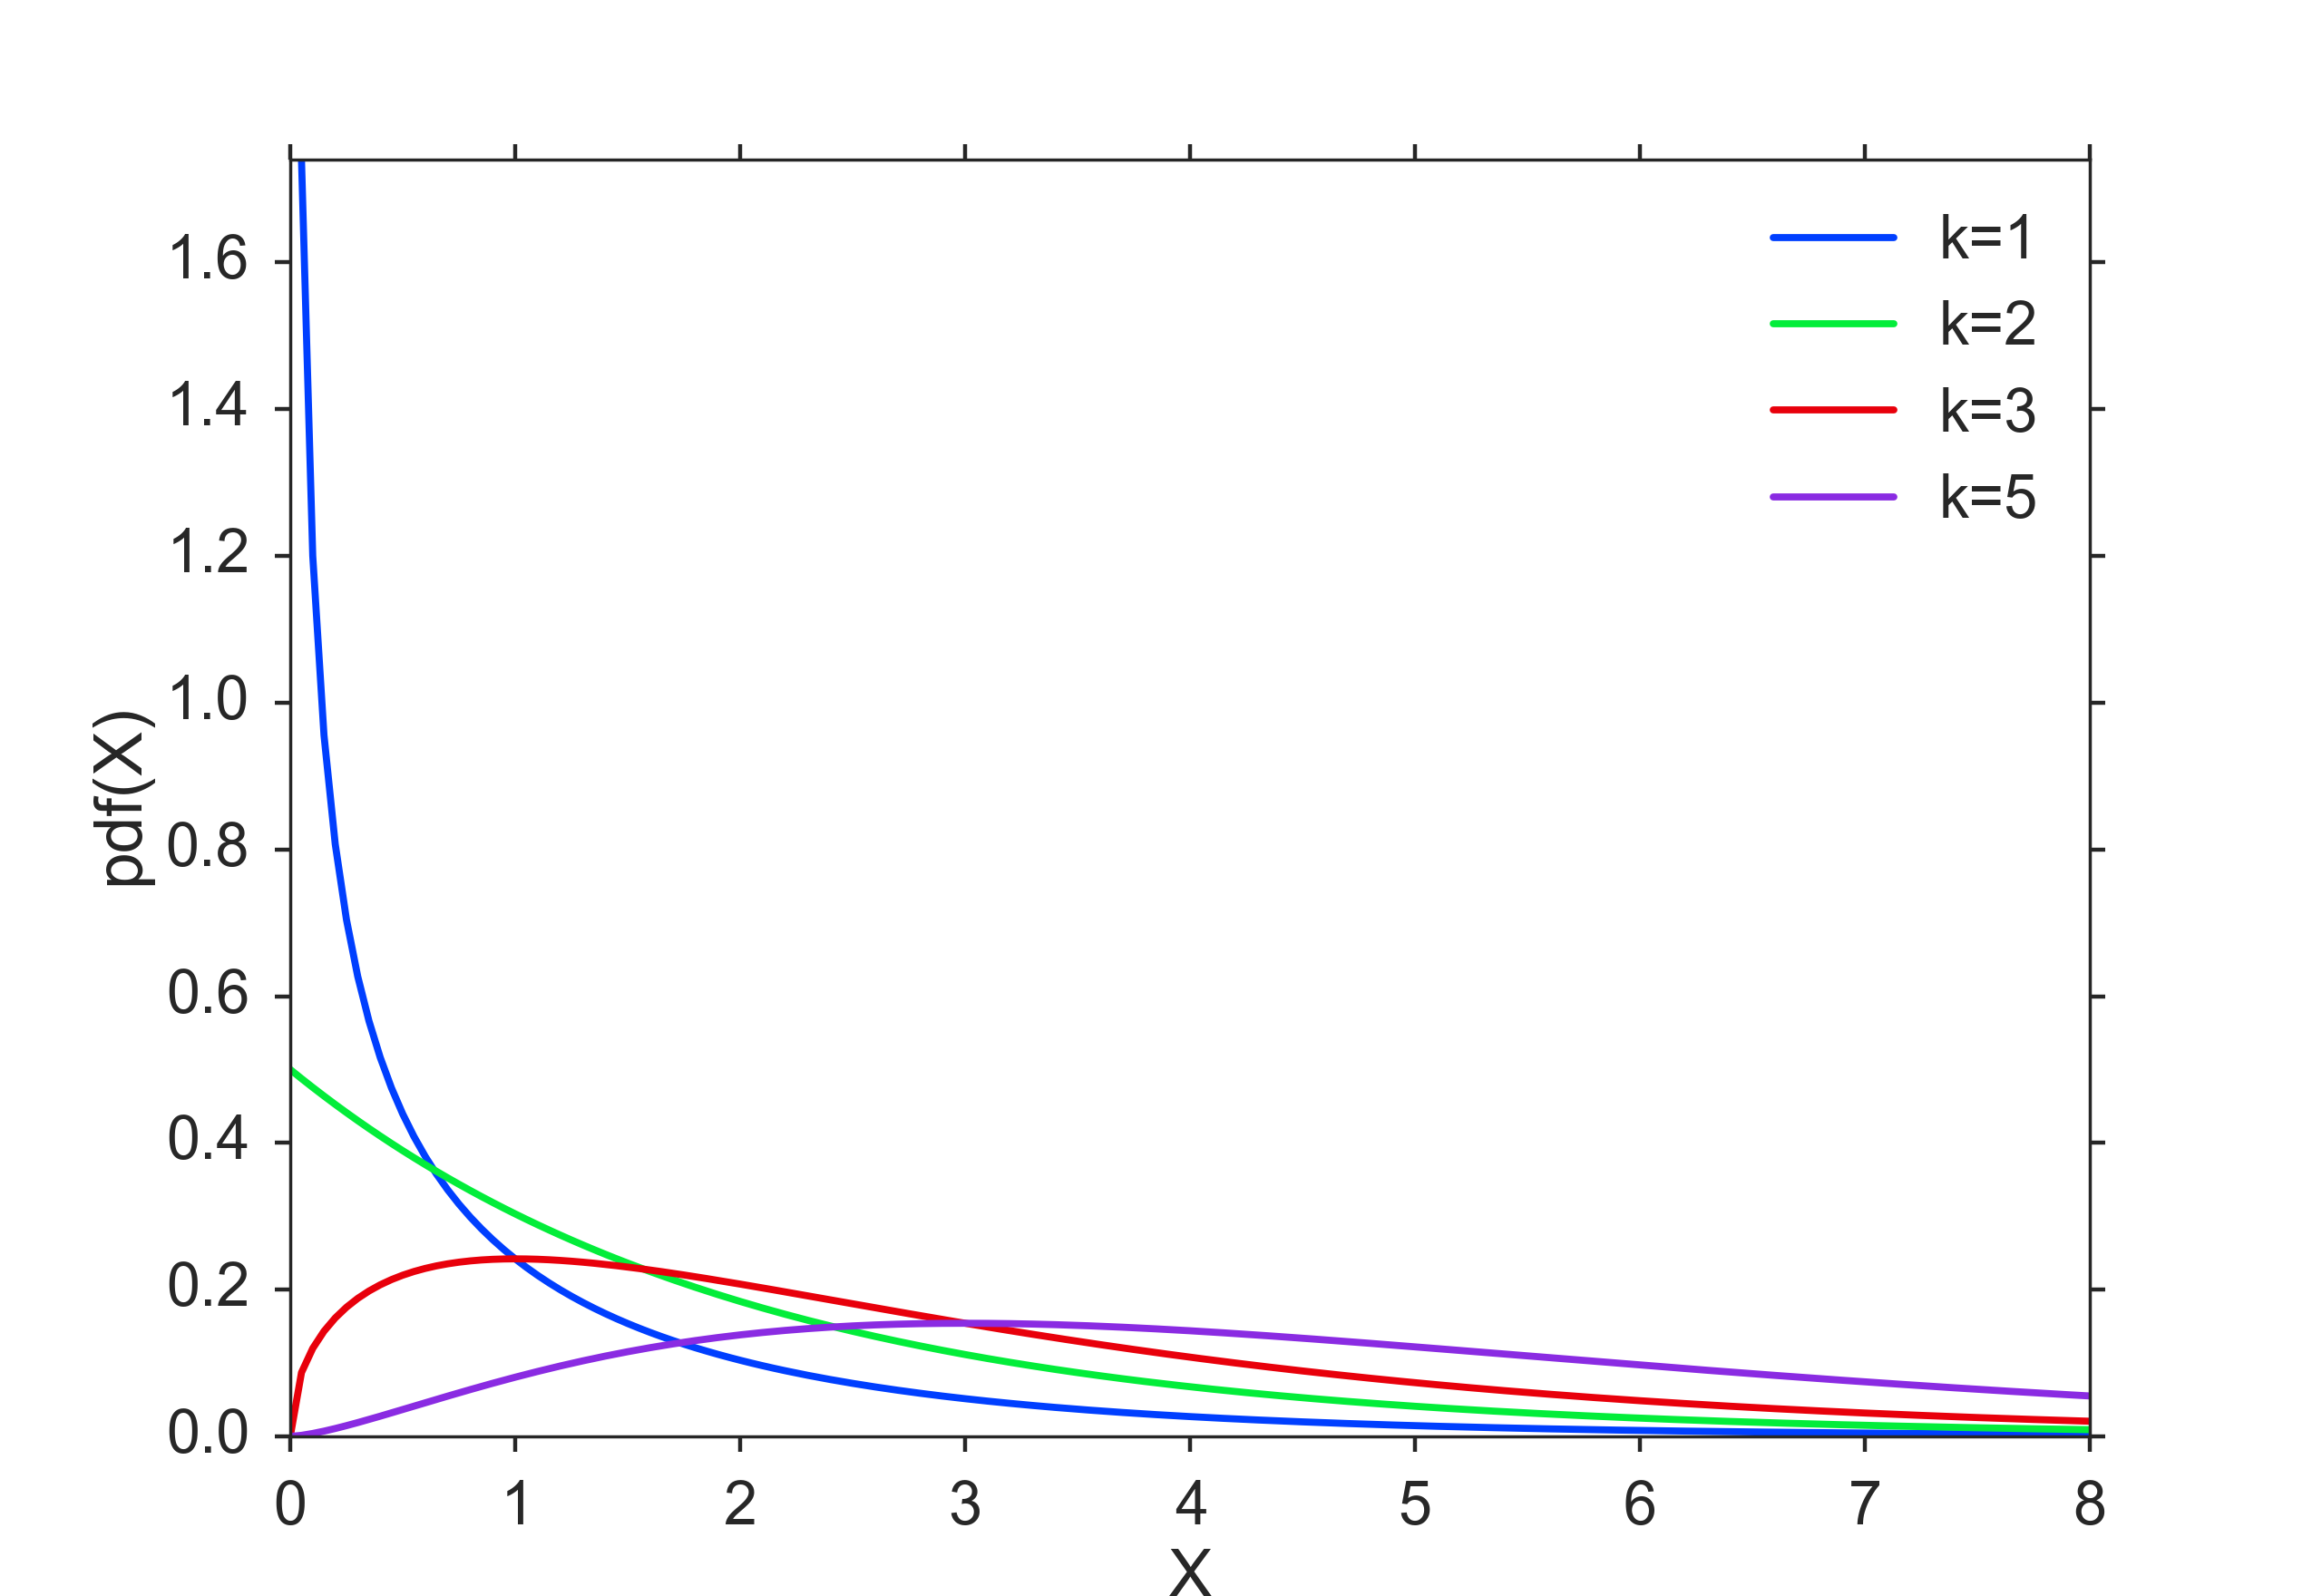
\includegraphics[width=0.5\textwidth]{../Images/dist_chi2.png}\\
  \caption{Chi-square Distribution}
  \label{fig:chi2}
\end{figure}

\textbf{Application Example}

A pill producer is ordered to deliver pills with a standard deviation of $\sigma=0.05$. From the next batch of pills you pick $n=13$ random samples. These samples $x_1, x_2, . . . , x_n$ have a weight of
3.04, 2.94, 3.01, 3.00, 2.94, 2.91, 3.02, 3.04, 3.09, 2.95, 2.99, 3.10, 3.02 g.

\emph{Question:} is the standard deviation larger than allowed?

\emph{Answer:}

Since the Chi-square distribution describes the distribution of the summed squares of random variates from a \emph{standard normal distribution}, we have to normalize our data before we calculate the corresponding CDF-value:

\begin{equation}
  1 - CD{F_{{\chi ^2}_{(n - 1)}}}\left( {\sum {(\frac{{x - \bar x}}{\sigma }} {)^2}} \right) = 0.1929
\end{equation}

\emph{Interpretation:} if the batch of pills is from a distribution with a standard deviation of $\sigma=0.05$, the likelihood of obtaining a chi-square value as large or larger than the one observed is about 19\%, so it is not atypical. In other words, the batch matches the expected standard deviation.

\subsubsection{F Distribution}\index{general}{distributions!F distribution}
Named after Sir Ronald Fisher, who developed the F distribution for use in determining critical values in ANOVAs (\emph{ANalysis Of VAriance}).
Suppose we want to calculate the variance of a variable in two separate subsets. "Is one more diverse than the other?" It is tempting to take the ratio of the variances, $S_1^2 / S_2^2$, but we don't know for sure how big or small that number must be before we conclude that the variances are different. This problem is solved by the F distribution. The cutoff values in an F table are found using three variables:

\begin{itemize}
  \item ANOVA numerator degrees of freedom
  \item ANOVA denominator degrees of freedom
  \item significance level
\end{itemize}

ANOVA compares the size of the variance between two different samples. This is done by dividing the larger variance over the smaller variance. The formula for the resulting \emph{F statistic} is (Fig. \ref{fig:Fdistribution}):

\begin{equation}
    F(r_1, r_2) = \frac{\chi_{r1} ^2 /r_1}{\chi_{r2} ^2 /r_2}
\end{equation}

where $\chi_{r1}^2$ and $\chi_{r2}^2$ are the chi-square statistics of sample one and two respectively, and $r_1$ and $r_2$ are their degrees of freedom, i.e. the number of observations.

\begin{figure}
  \centering
  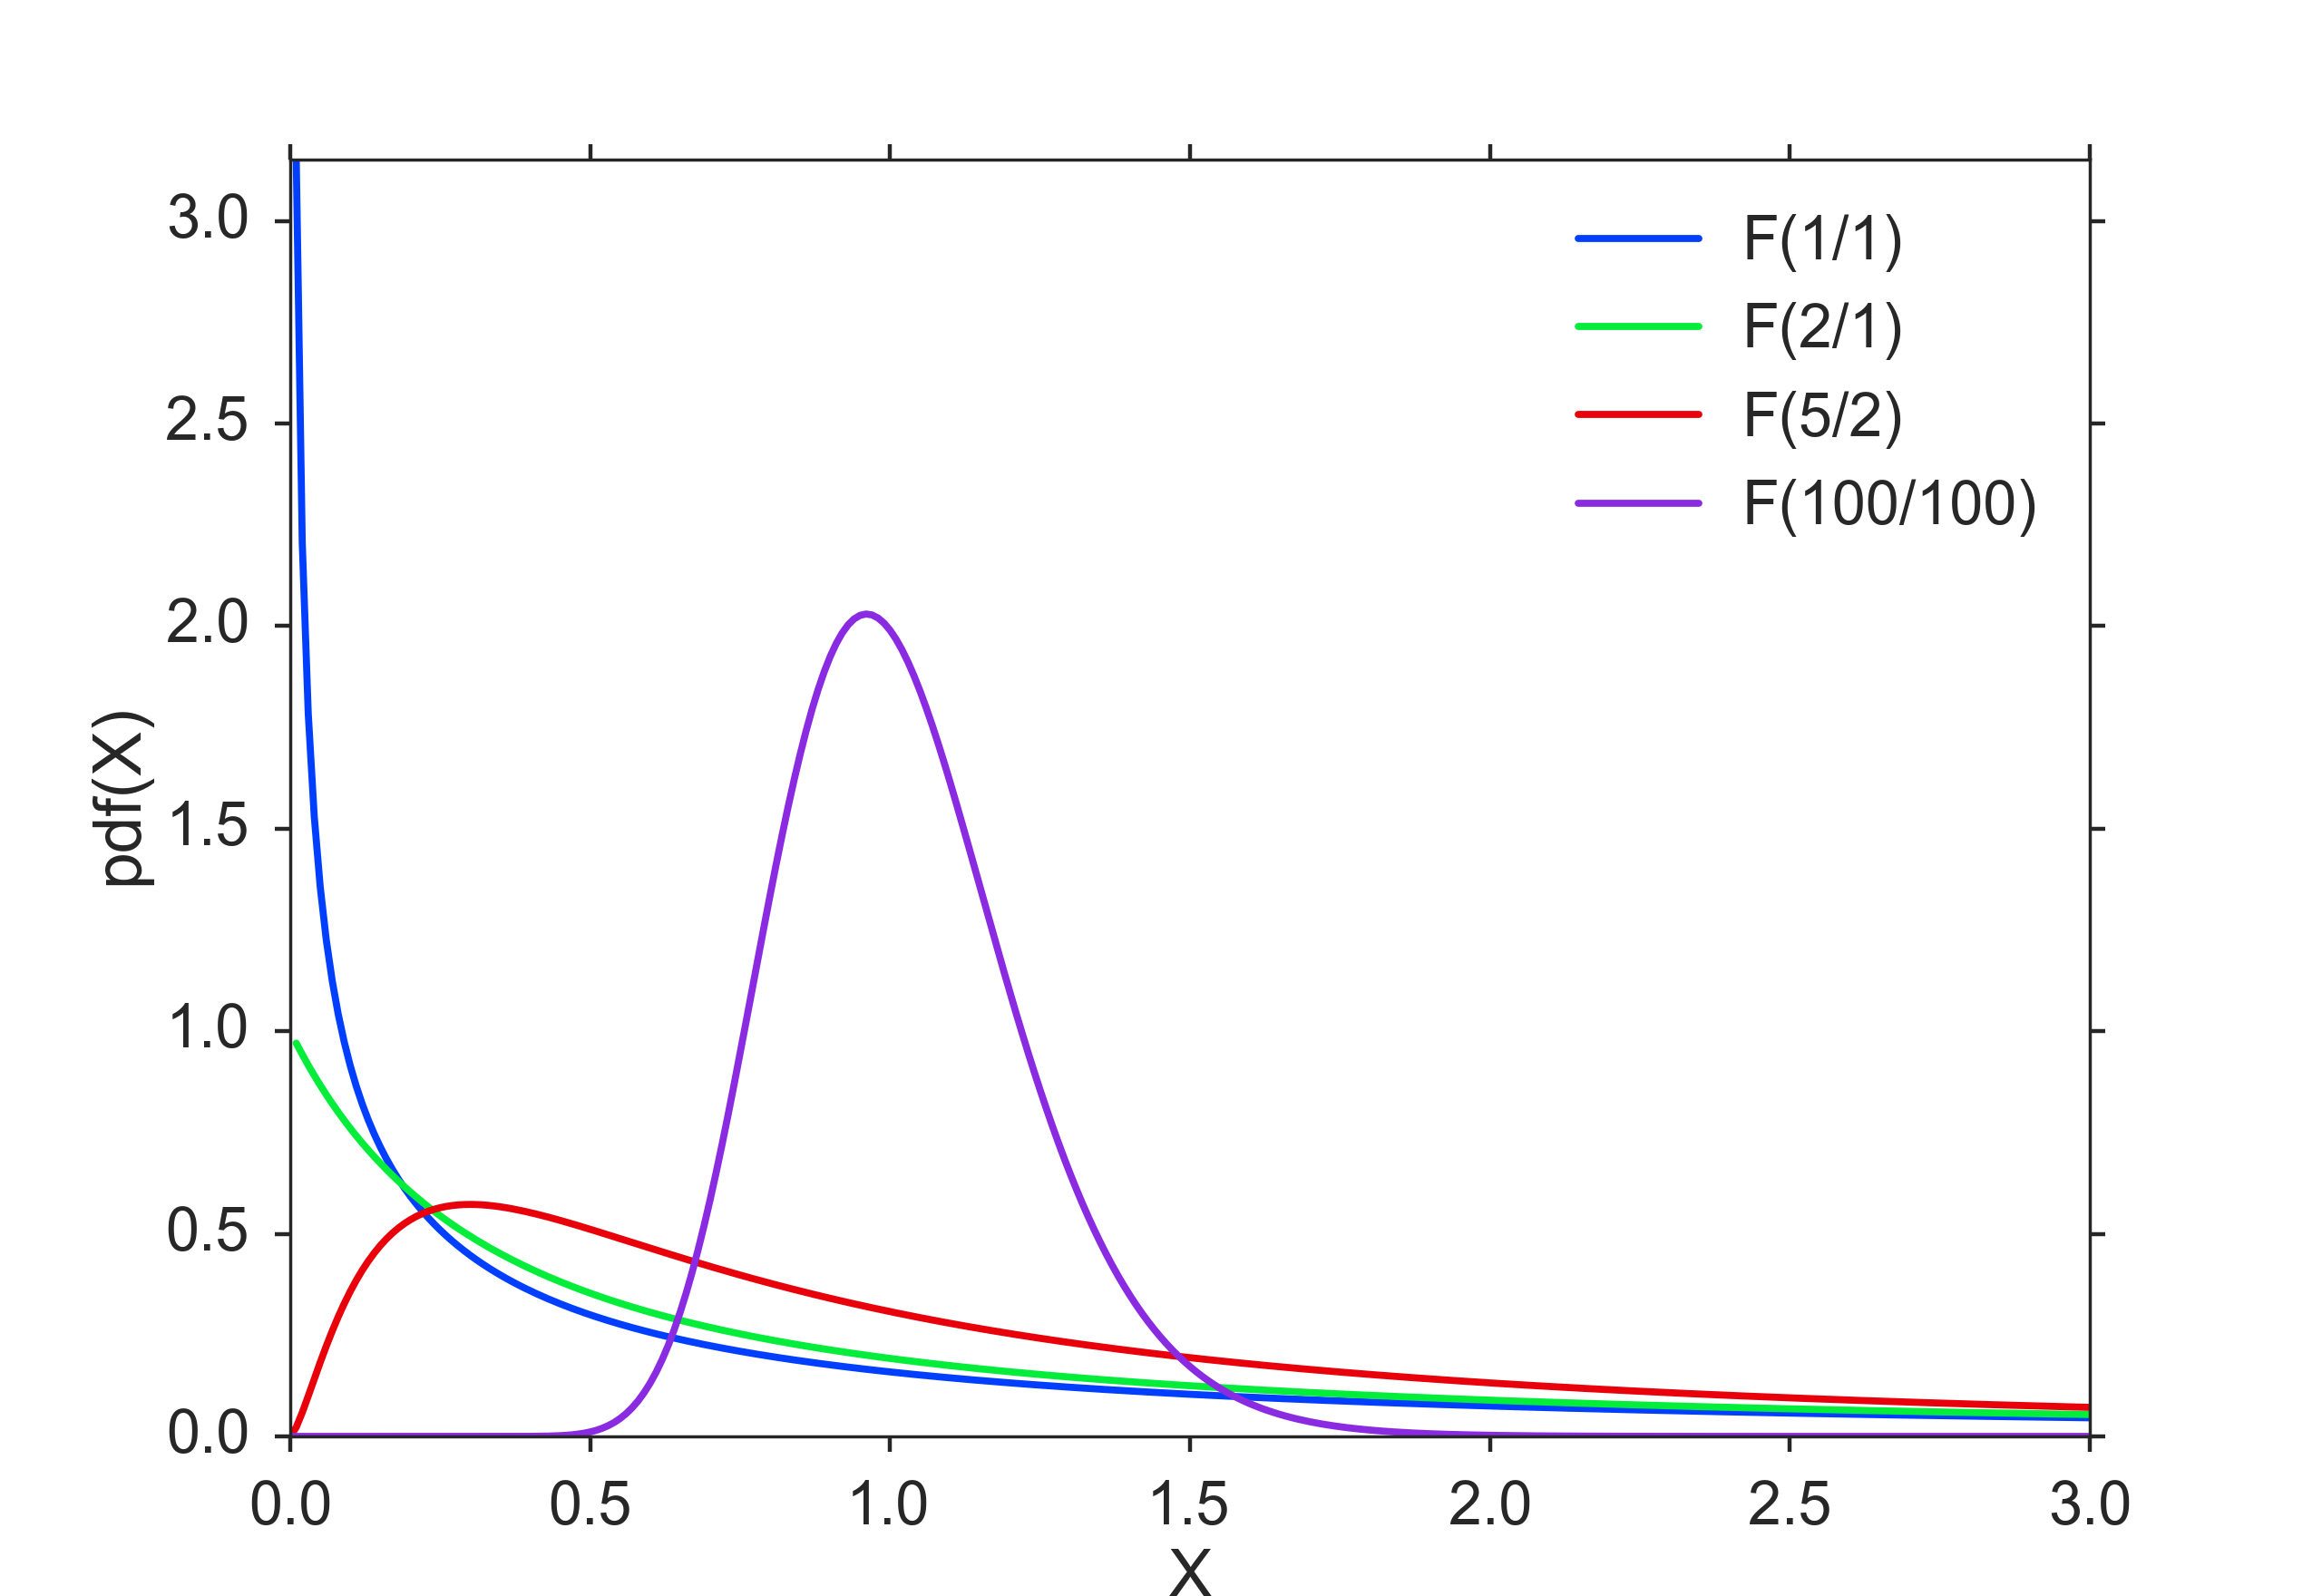
\includegraphics[width=0.5\textwidth]{../Images/dist_f.png}\\
  \caption{F Distribution}
  \label{fig:Fdistribution}
\end{figure}


\paragraph{F-Test of Equality of Variances}
If you want to investigate whether two groups have the same variance, you have to calculate the ratio of the sample standard deviations squared:

\begin{equation}
  F = \frac{S_x^2}{S_y^2}
\end{equation}

where $S_x$ ist he sample standard deviation of the first sample, and $S_y$ the sample standard deviation for the second sample.

\textbf{Application Example}

Take for example the case that you want to compare two methods to measure eye movements. The two methods
can have different accuracy and different precision (Fig. \ref{fig:accuracy}). With your test you want to
determine if the precision of the two methods is equivalent, or if one
method is more precise than the other.

\begin{figure}
  \centering
  \includegraphics[width=0.5\textwidth]{../Images/Accuracy_and_precision.png}\\
  \caption{Accuracy and precision of a measurement are two different characteristics!}
  \label{fig:accuracy}
\end{figure}

When you look 20 deg to the right, you get the following results:
Method 1: [20.7,  20.3,  20.3,  20.3,  20.7,  19.9,  19.9,  19.9,  20.3,
        20.3,  19.7,  20.3]
Method 2: [ 19.7,  19.4,  20.1,  18.6,  18.8,  20.2,  18.7,  19. ]

The F statistic is $F = 0.494$, and has $n-1$ and $m-1$ degrees of freedom, where $n$ and $m$ are the number of recordings with each method. The code sample below shows that the F statistic is close to the center of the distribution, so we cannot reject the hypothesis that the two methods have the same precision.

\begin{lstlisting}
  In [1]:  method1 = array([20.7,  20.3,  20.3,  20.3,  20.7,  19.9,  19.9,  19.9,  20.3,
        20.3,  19.7,  20.3])
  In [2]:  method2 = array([ 19.7,  19.4,  20.1,  18.6,  18.8,  20.2,  18.7,  19. ])
  In [3]:  fval = var(method1, ddof=1)/var(method2, ddof=1)
  In [4]:  fd = stats.f(len(method2)-1,len(method2)-1)
  In [5]:  p = fd.cdf(fval)
  In [6]:  print p
  Out[6]:  0.041
  In [7]:  if (p<0.025) or (p>0.975):
              print 'There is a significant difference between the two distributions.'
\end{lstlisting}


\subsubsection{Lognormal Distribution}\index{general}{distributions!lognormal}

Normal distributions are the easiest ones to work with. In some circumstances a set of data with a positively skewed distribution can be transformed into a symmetric, normal distribution by taking logarithms. Taking logs of data with a skewed distribution will often give a distribution that is near to normal (see Figure \ref{fig:lognormal}).

\begin{figure}
\centering
\begin{subfigure}{.5\textwidth}
  \centering
  \includegraphics[width=.8\linewidth]{../Images/LogNormal_Linear.png}
  \caption{Plotted against a linear abscissa.}
  \label{fig:Lognormal_Sub1}
\end{subfigure}%
\begin{subfigure}{.5\textwidth}
  \centering
  \includegraphics[width=.8\linewidth]{../Images/LogNormal_Logarithmic.png}
  \caption{Plotted against a logarithmic abscissa.}
  \label{fig:Lognormal_Sub2}
\end{subfigure}
\caption{Lognormal distribution}
\label{fig:lognormal}
\end{figure}

\subsubsection{Weibull Distribution}\index{general}{distributions!weibull}

The Weibull distribution is the most commonly used distribution for modeling reliability data or "survival" data. It has two parameters, which allow it to handle increasing, decreasing or constant failure-rates (see Figure \ref{fig:weibull}).
It is defined as

\begin{equation}\label{eq_weibull}
f_x (x) =
  \begin{cases}
    \frac{k}{\lambda}\left(\frac{x}{\lambda}\right)^{k-1}e^{-(x/\lambda)^{k}} & x\geq0 ,\\
    0 & x<0 ,
    \end{cases}
\end{equation}

where $k > 0$ is the \emph{shape parameter }and $\lambda > 0$ is the \emph{scale parameter }of the distribution. Its complementary cumulative distribution function is a stretched exponential function.

If the quantity x is a "time-to-failure", the Weibull distribution gives a distribution for which the failure rate is proportional to a power of time. The shape parameter, k, is that power plus one, and so this parameter can be interpreted directly as follows:

\begin{itemize}
  \item  A value of $k < 1$ indicates that the failure rate decreases over time. This happens if there is significant "infant mortality", or defective items failing early and the failure rate decreasing over time as the defective items are weeded out of the population.

  \item  A value of $k = 1$ indicates that the failure rate is constant over time. This might suggest random external events are causing mortality, or failure.
  \item  A value of $k > 1$ indicates that the failure rate increases with time. This happens if there is an "aging" process, or parts that are more likely to fail as time goes on.
\end{itemize}

In the field of materials science, the shape parameter k of a distribution of strengths is known as the Weibull modulus.

\begin{figure}
  \centering
  \includegraphics[width=0.5\textwidth]{../Images/Weibull_PDF.png}\\
  \caption{Weibull Distribution}\label{fig:weibull}
\end{figure}


\subsubsection{Exponential Distribution}\index{general}{distributions!exponential}

For a stochastic variable X with an \emph{exponential distribution}, the probability distribution function is:
\begin{equation}\label{eq_exponential}
f_x (x) =
  \begin{cases}
\lambda e^{- \lambda x}, & \mbox{if } x \ge 0 \\
0, & \mbox{if } x < 0
\end{cases}
\end{equation}

The exponential PDF is shown in Figure \ref{fig:exponential}
\begin{figure}
  \centering
  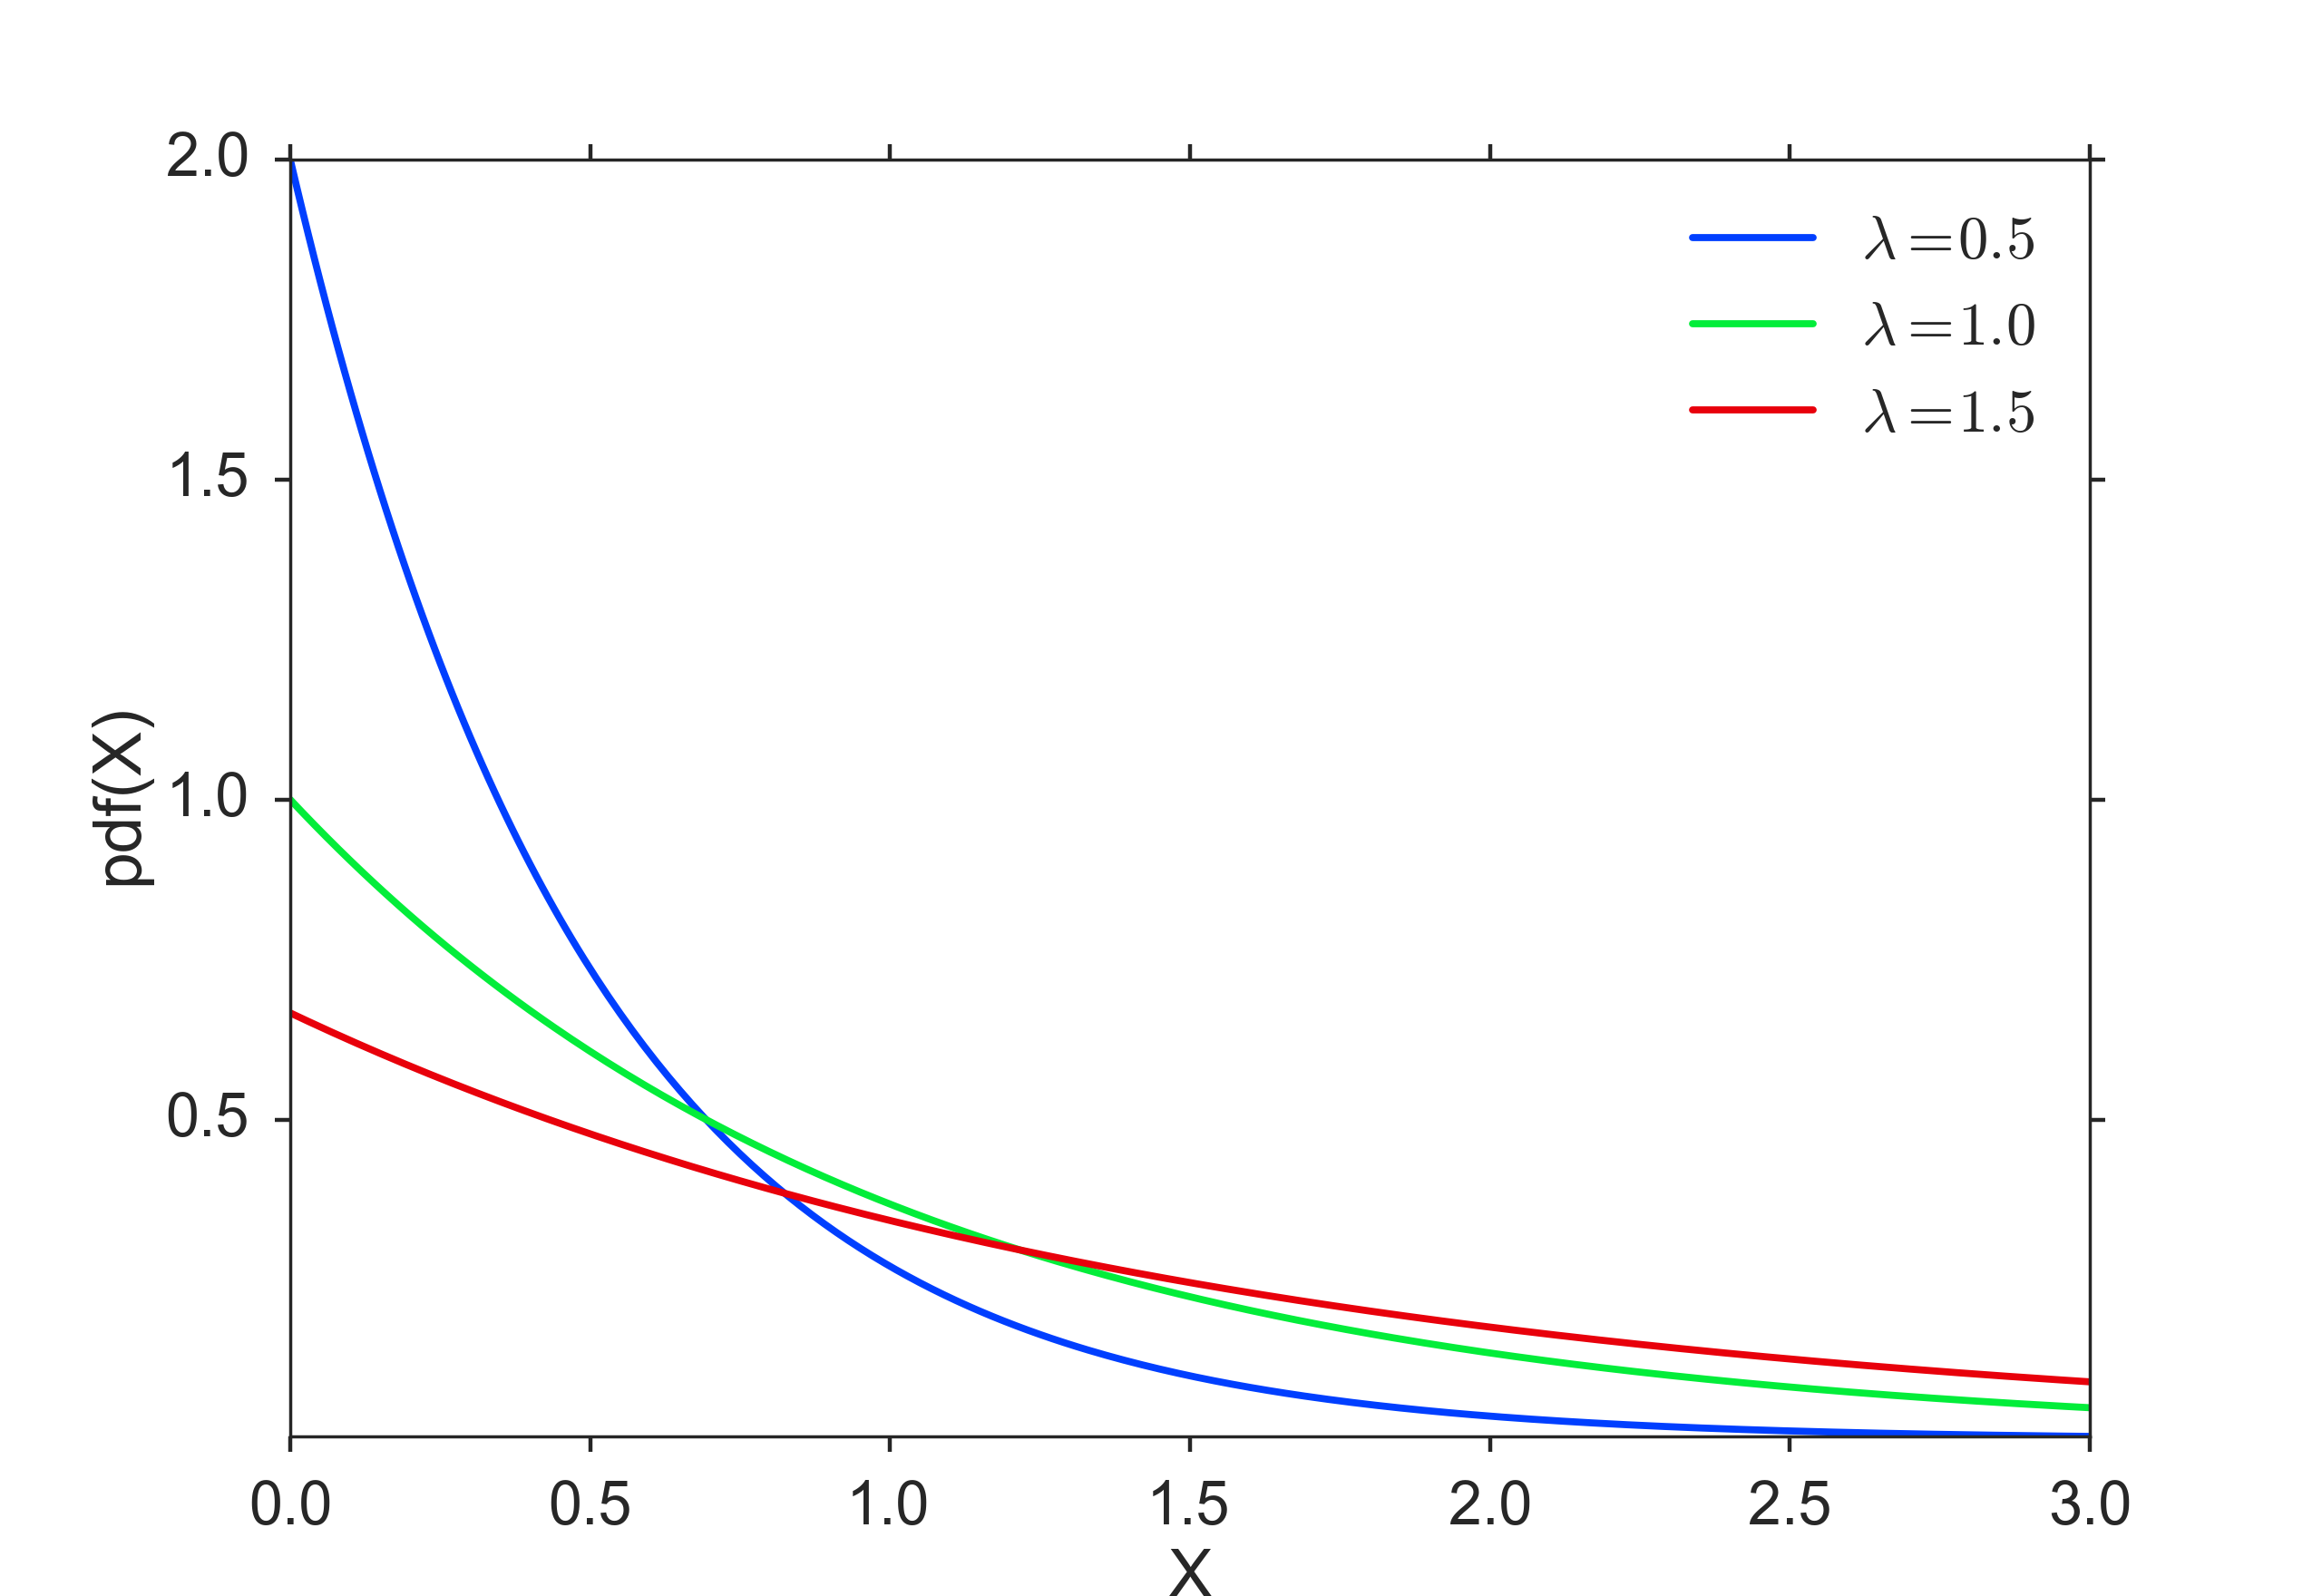
\includegraphics[width=0.5\textwidth]{../Images/dist_exp.png}\\
  \caption{Exponential Distribution}\label{fig:exponential}
\end{figure}


\subsubsection{Uniform Distribution}\index{general}{distributions!uniform}

This is a simple one: an even probability for all data values (Figure \ref{fig:uniform}). Not very common for real data.

\begin{figure}
  \centering
  \includegraphics[width=0.5\textwidth]{../Images/Uniform_Distribution_PDF.png}\\
  \caption{Uniform Distribution} \label{fig:uniform}
\end{figure}

\subsubsection{Programs: Continuous Distribution Functions}

Working with distribution functions in Python takes a bit to get used to. But once you get the concept, it is marvellously easy. In my opinion, the most logical way is first to define the function, with all the parameters that it requires; and then, to use the methods of this function, e.g. $pdf$, or $cdf$:

\begin{lstlisting}
  In [1]: from scipy import stats
  In [2]: myDF = stats.norm(5,3)
  In [3]: x = linspace(-5, 15, 101)
  In [4]: y = myDF.pdf(x)
\end{lstlisting}

\PyImg "distributionContinuous.py" (p \pageref{py:continuous}) shows different continuous distribution functions.
\index{python}{distributionContinuous}

\subsection{Discrete Distributions}\index{general}{distributions!discrete}

While the functions describing continuous distributions are referred to as \emph{probability density functions}, discrete distributions are described by \emph{probability mass functions}.

Two discretely distributions are commonly encountered: the \emph{binomial distribution}, and the \emph{Poisson distribution}. These two have the following properties:

\begin{table}[h]
  \centering
  \begin{tabular}{l|c|c|}
      & Mean & Variance \\
      \hline
      Binomial & $n \cdot p$ & $np(1-p)$ \\
      Poisson & $\lambda$ & $\lambda$ \\
      %\hline
  \end{tabular}
\caption{Properties of discrete distributions.}
\end{table}

The big difference between those two functions that you have to keep in mind: applications of the Binomial function have an inherent upper limit (e.g. when you throw dice five times, each side can come up a maximum of five times); in contrast, the Poisson distribution does not have an inherent upper limit (e.g. how many people you know).

\subsubsection{Binomial Distribution}\index{general}{distributions!binomial}\label{sec:binomialDist}
The Binomial is associated with the question "Out of a given (fixed) number of trials, how many will succeed?" Some example questions that are modeled with a Binomial distribution are:
\begin{itemize}
  \item Out of ten tosses, how many times will this coin land ''heads''?
  \item From the children born in a given hospital on a given day, how many of them will be girls?
  \item How many students in a given classroom will have green eyes?
  \item How many mosquitos, out of a swarm, will die when sprayed with insecticide?
\end{itemize}

  We conduct $n$ repeated experiments where the probability of success is given by the parameter $p$ and add up the number of successes. This number of successes is represented by the random variable $X$.  The value of $X$ is then between 0 and $n$.

When a random variable X has a Binomial Distribution with parameters $p$ and $n$ we write it as $\,X \sim B(n,p)$ and the probability mass function is given at $X=k$ by the equation:

\begin{equation}
    P\left[X = k\right] = \begin{cases} {n \choose k} p^k \left(1-p\right)^{n-k}\ & 0 \le k \le n \\ 0 & \mbox{otherwise} \end{cases} \quad 0 \leq p \leq 1, \quad n \in \mathbb{N}
\end{equation}

where ${n \choose k}={n! \over k!(n-k)!}$

\begin{figure}
  \centering
  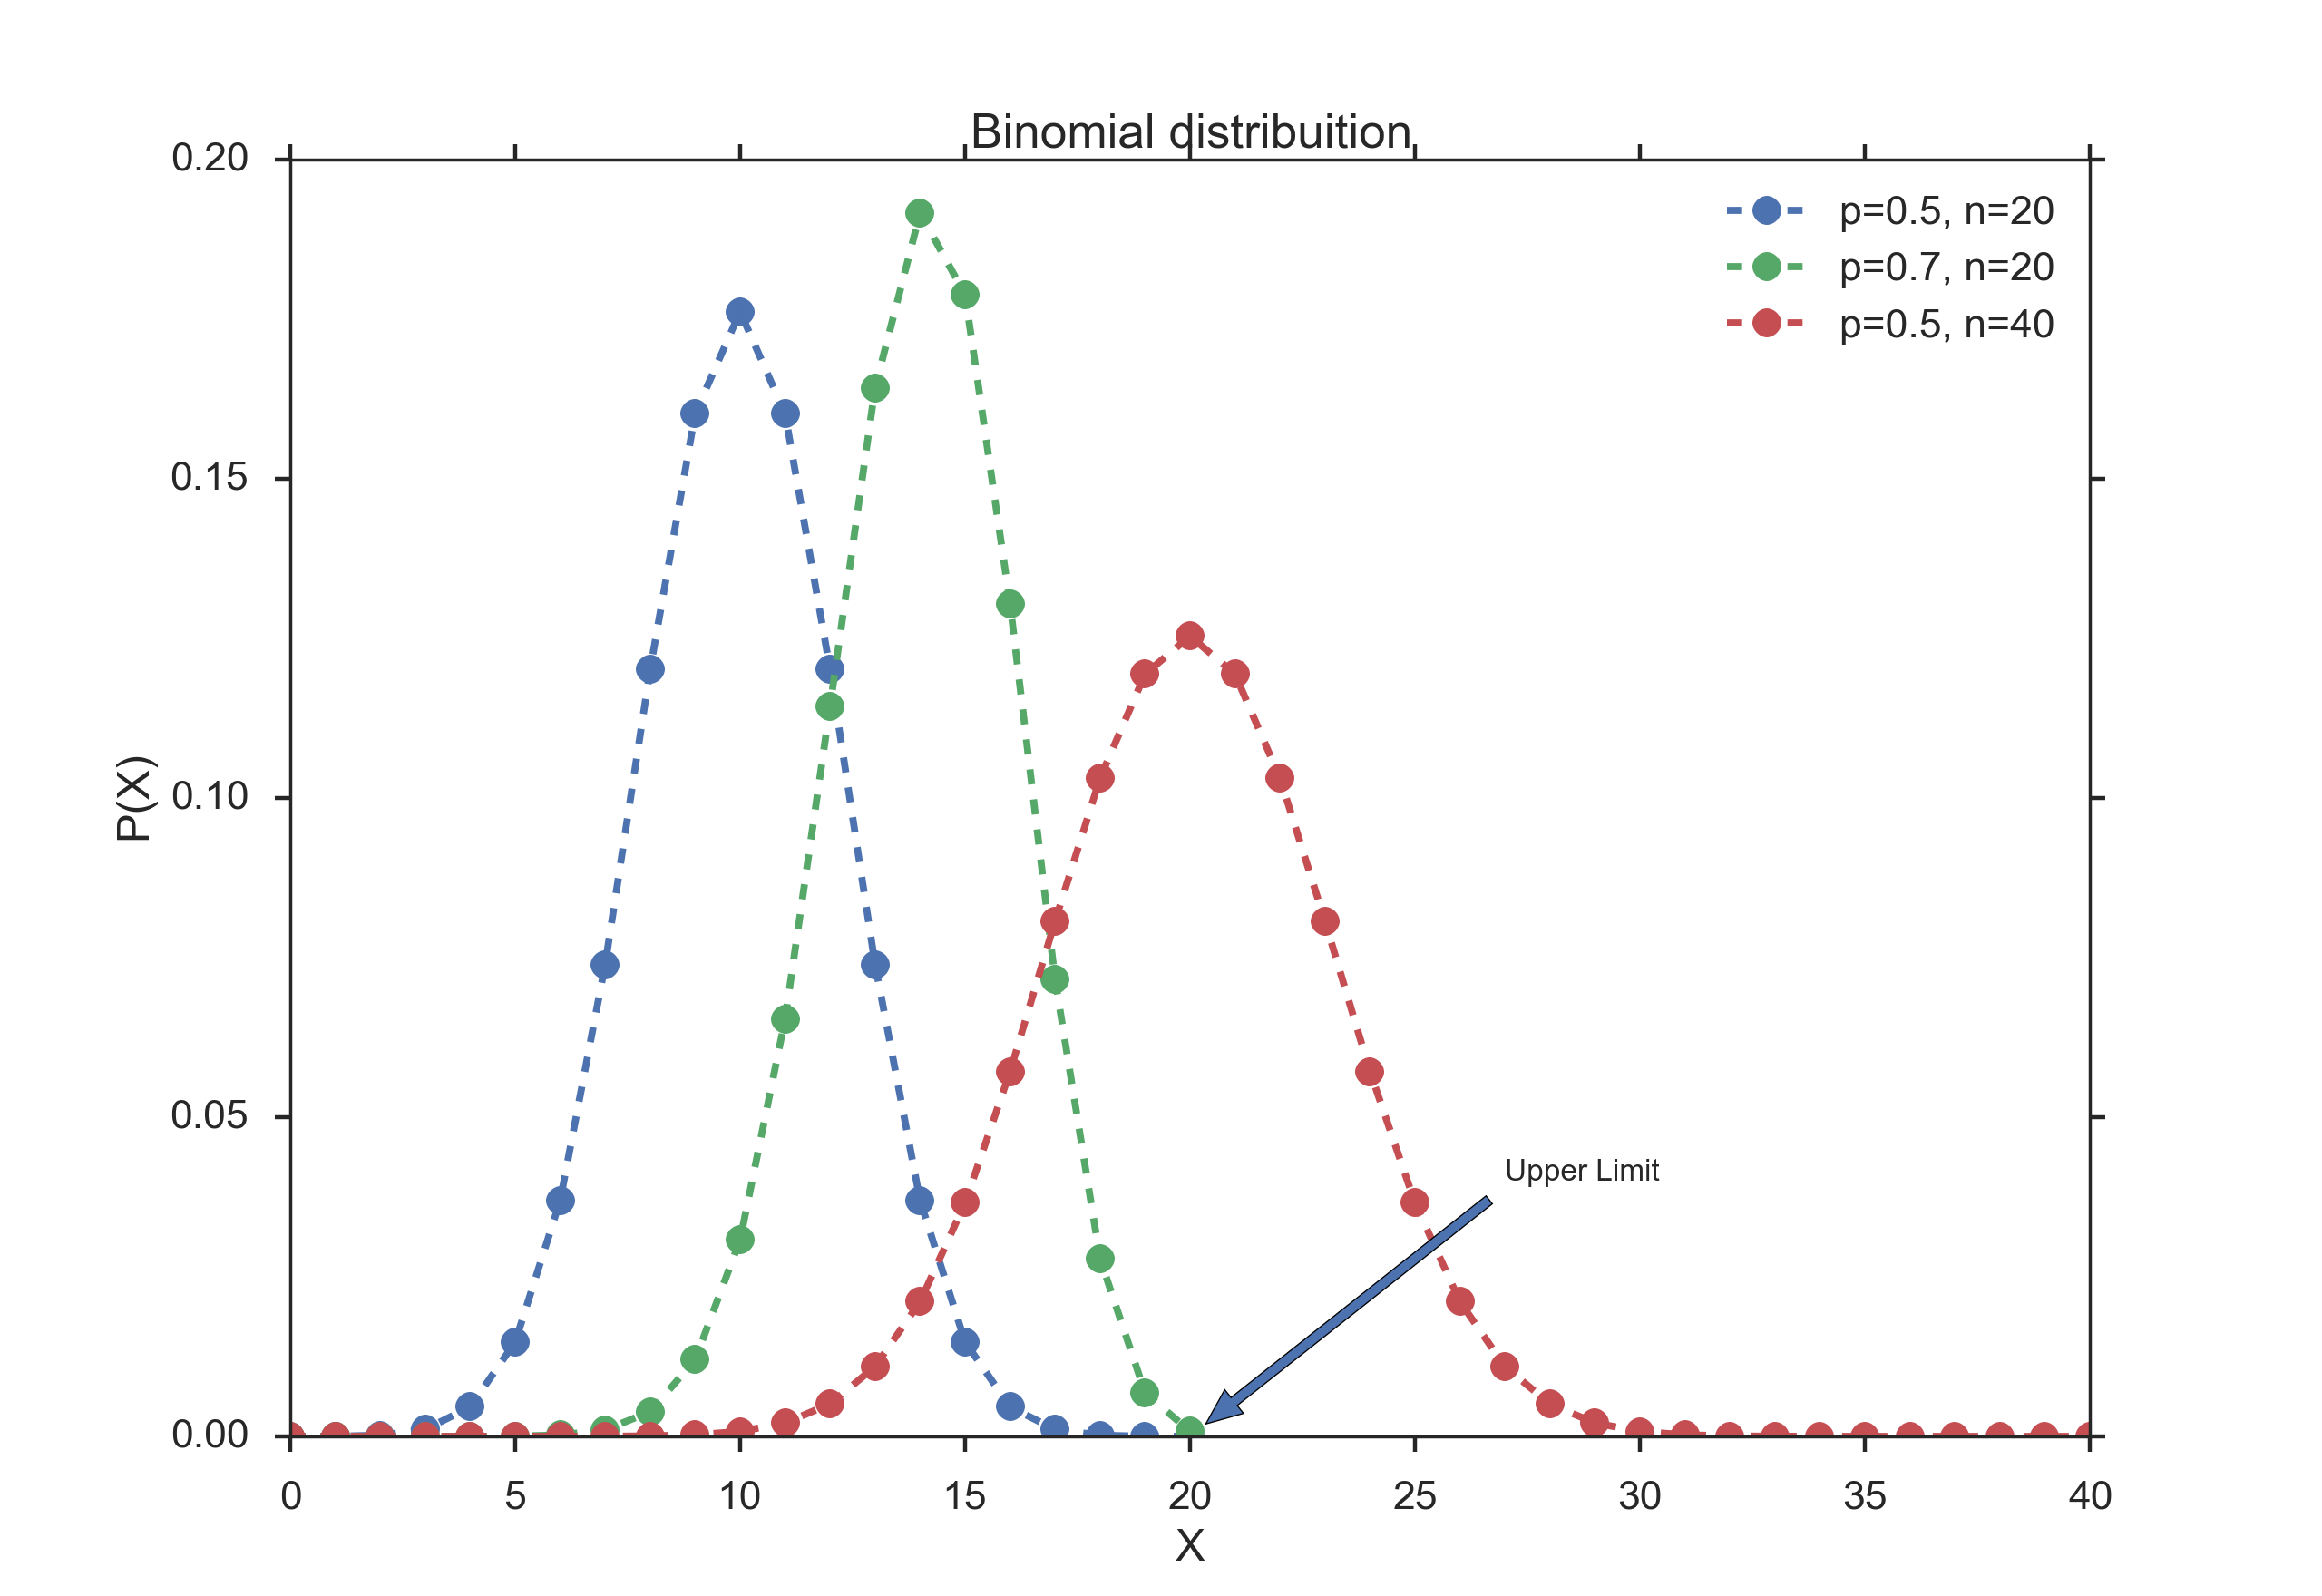
\includegraphics[width=0.66\textwidth]{../Images/Binomial_distribution_pmf.png}\\
  \caption{Binomial Distribution. Note that legal values exist only for integer x. The dotted lines in between only facilitate the grouping of the values to individual distribution parameters.}
\end{figure}

The binomial distribution for $n = 1$ is sometimes referred to as \emph{Bernoulli Distribution}\index{general}{distributions!Bernoulli}.

 For $n$ trials, we have the following properties:

 \begin{itemize}
   \item mean: $np$
   \item variance: $n p (1-p)$
 \end{itemize}

\paragraph{Example: Binomial Test}\index{general}{test!binomial}

Suppose we have a board game that depends on the roll of a die and attaches special importance to rolling a 6. In a particular game, the die is rolled 235 times, and 6 comes up 51 times. If the die is fair, we would expect 6 to come up 235/6 = 39.17 times. Is the proportion of 6's significantly higher than would be expected by chance, on the null hypothesis of a fair die?

To find an answer to this question using the \emph{Binomial Test}, we consult the binomial distribution with n=235 and p=1/6, to determine the probability of finding exactly 51 sixes in a sample of 235 if the true probability of rolling a 6 on each trial is 1/6. We then find the probability of finding exactly 52, exactly 53, and so on up to 235, and add all these probabilities together. In this way, we calculate the probability of obtaining the observed result (51 6s) or a more extreme result ($>51 6's$) assuming that the die is fair. In this example, the result is 0.0265, which indicates that observing 51 6's is unlikely (significant at the 5\% level) to come from a die that is not loaded to give many 6's (one-tailed test).

Clearly a die could roll too few sixes as easily as too many and we would be just as suspicious, so we should use the two-tailed test which (for example) splits the 5\% probability across the two tails.

\PyImg "binomial.py" (p \pageref{py:binomial}): Example of a one-and two-sided binomial test.
\index{python}{binomialTest}


\subsubsection{Poisson Distribution}\index{general}{distributions!poisson}

Any French speaker will notice that "Poisson" means "fish", but really there's nothing fishy about this distribution. It's actually pretty straightforward. The name comes from the mathematician Siméon-Denis Poisson (1781-1840).

The Poisson Distribution is ''very similar'' to the Binomial Distribution. We are examining the number of times an event happens. The difference is subtle. Whereas the Binomial Distribution looks at how many times we register a success over a fixed total number of trials, the Poisson Distribution measures how many times a discrete event occurs, over a period of continuous space or time. There is no "total" value n. As with the previous sections, let's examine a couple of experiments or questions that might have an underlying Poisson nature.

\begin{itemize}
  \item How many pennies will I encounter on my walk home?
  \item How many children will be delivered at the hospital today?
  \item How many products will I sell after airing a new television commercial?
  \item How many mosquito bites did you get today after having sprayed with insecticide?
  \item How many defects will there be per 100 metres of rope sold?
\end{itemize}

What's a little different about this distribution is that the random variable $X$ which counts the number of events can take on \emph{any non-negative integer} value. In other words, I could walk home and find no pennies on the street. I could also find one penny. It's also possible (although unlikely, short of an armored-car exploding nearby) that I would find 10 or 100 or 10,000 pennies.

Instead of having a parameter p that represents a component probability like in the Binomial distribution, this time we have the parameter "lambda" or $\lambda$ which represents the "average or expected" number of events to happen within our experiment. The probability mass function of the Poisson is given by

\begin{equation}
  P(X=k)=\frac{e^{-\lambda}\lambda^k}{k!}
\end{equation}.

The Poisson distribution has the following properties:

\begin{itemize}
    \item mean: $\lambda$
    \item variance: $\lambda$
\end{itemize}

\begin{figure}
  \centering
  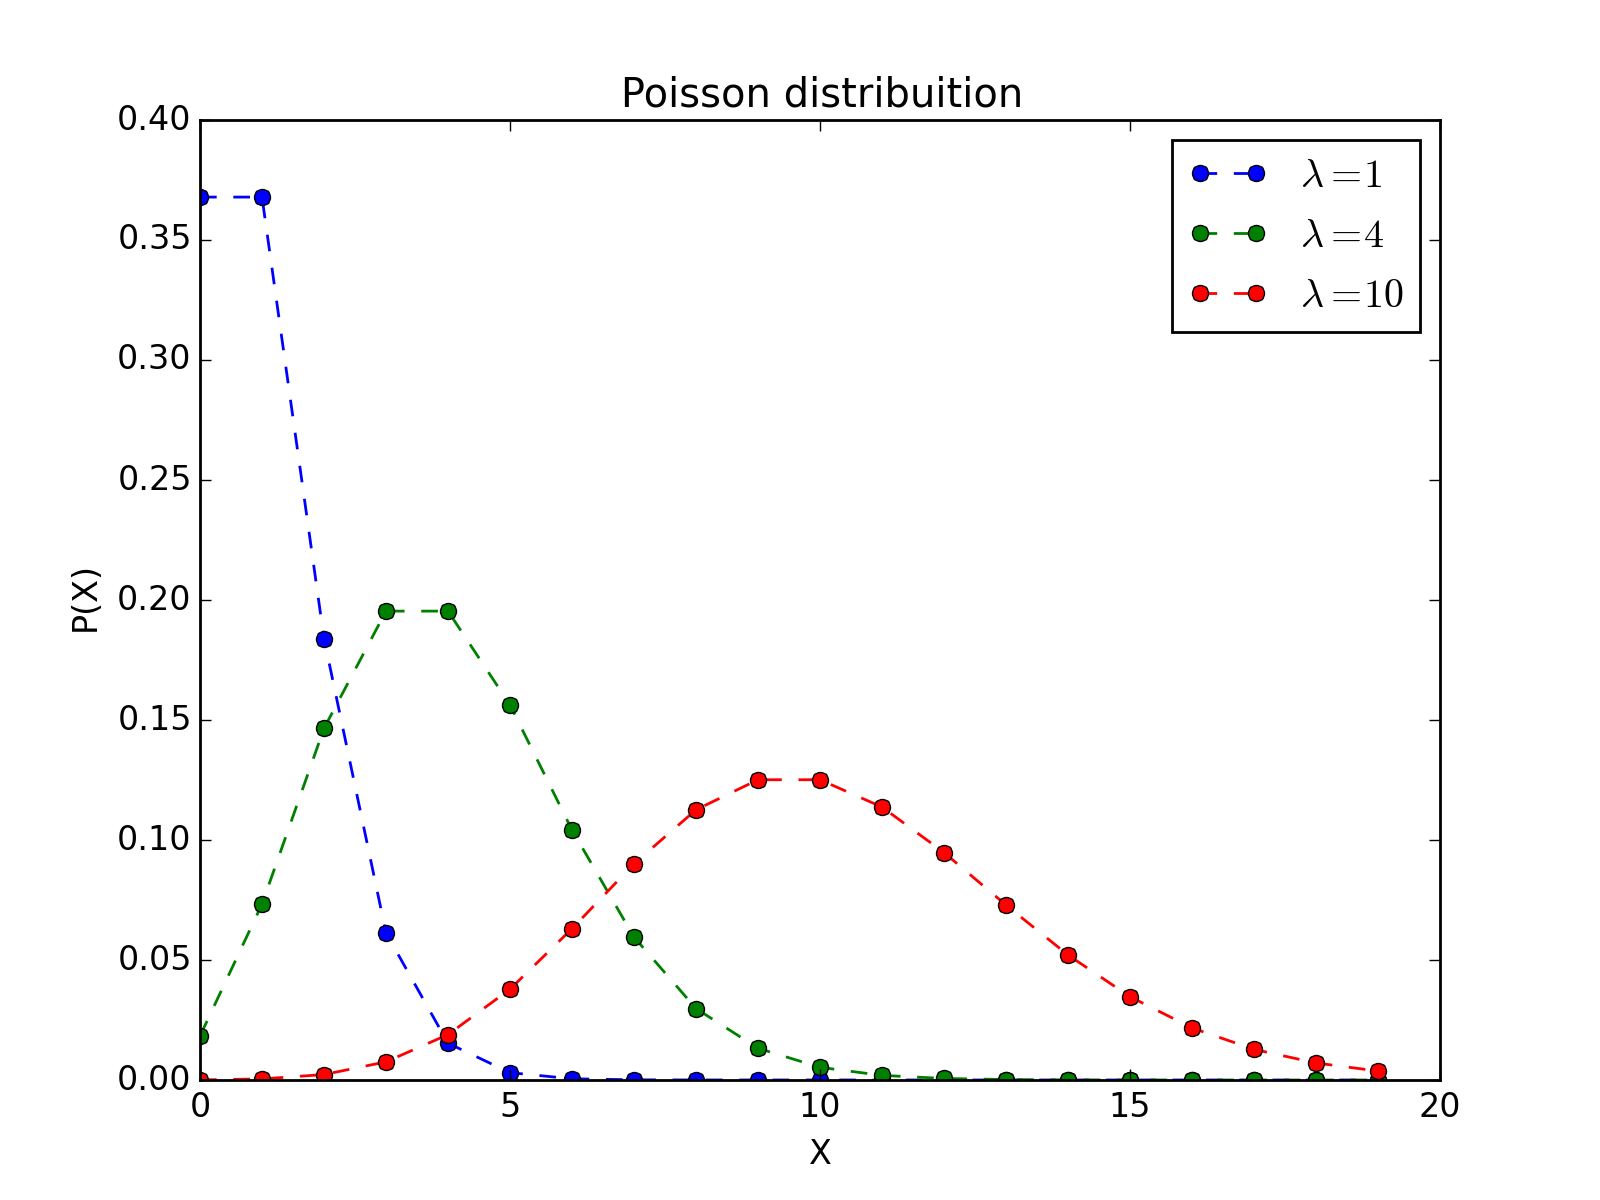
\includegraphics[width=0.66\textwidth]{../Images/Poisson_distribution_pmf.png}\\
  \caption{Poisson Distribution. Again note that legal values exist only for integer x. The dotted lines in between only facilitate the grouping of the values to individual distribution parameters.}
\end{figure}

\subsubsection{Programs: Discrete Distribution Functions} \index{general}{distributions!discrete}

\PyImg "distributionDiscrete.py" (p \pageref{py:discrete}) shows different continuous distribution functions.
\index{python}{distributionDiscrete}
%(Lecture 7)

\section{Exercises}

\subsection*{Python}
\begin{enumerate}
  \item Create an numpy-array, containing the data 1,2,3,...,10. Calculate mean and sample(!)-standard deviation.
    (Correct answer: 3.03)
\end{enumerate}

\subsection*{Distributions}


\begin{enumerate}
  \item  Generate and plot the Probability Density Function (PDF) of a normal distribution, with a mean of 5 and a standard deviation of 3.
  \item  Generate 1000 random data from this distribution.
  \item  Calculate the standard error of the mean of these data.
    (Correct answer: ca. 0.096)

  \item  Plot the histogram of these data.
  \item  From the PDF, calculate the interval containing 95\% of these data.
    (Correct answer: [ -0.88, 10.88])
\end{enumerate}

\subsection*{Continuous Distributions }
\begin{enumerate}
    \item \textbf{Normal Distribution:} Your doctor tells you that he can use hip implants for surgery even if they are 1 mm bigger or smaller than the specified size. And your financial officer tells you that you can discard 1 out of 1000 hip implants, and still make a profit.

        What is the required standard deviation for the producer of the hip implants, to simultaneously satisfy both requirements?
        (Correct answer: $\sigma=0.304 mm$)
    \item \textbf{T-Distribution:} Measuring the weight of your colleagues, you have obtained the following weights: 52, 70, 65, 85, 62, 83, 59 kg.
    Calculate the corresponding mean, and the 99\% confidence interval for the mean. Note: with n values you have n-1 DOF for the t-distribution.
    (Correct answer: 68.0 +/- 17.2 kg)

    \item \textbf{Chi-square Distribution:} Create 3 normally distributed datasets (mean = 0, SD = 1), with 1000 samples each. Then square them, sum them (so that you have 1000 data-points), and create a histogram with 100 bins. This should be similar to the curve for the Chi-square distribution, with 3 DOF (i.e. it should come down at the left, see figure below).
    \begin{figure}
      \centering
      \includegraphics[width=0.5\textwidth]{../Images/chi2_3dof.png}\\
      \caption{chi2 distribution with 3 degrees of freedom.}\label{fig:chi23dof}
    \end{figure}

    \item \textbf{F Distribution:} You have two apple trees. There are three apples from the first tree that weigh 110, 121 and 143 grams respectively, and four from the other which weigh 88, 93, 105 and 124 grams respectively. Are the variances from the two trees different?
    Note: calculate the corresponding F-value, and check if the CDF for the corresponding F-distribution is $<0.025$.
    (Correct answer: no)
\end{enumerate}
\subsection*{Discrete Distributions }

\begin{enumerate}

    \item Under which conditions do you use the \emph{binomial distribution} to evaluate the likelihood of a discrete number of events? And under which do you use the \emph{Poisson distribution}?

    \item \textbf{Binomial Distribution} "According to research, pure blue eyes in Europe approach greatest frequency in Finland, Sweden and Norway(at 72\%), followed by Estonia, Denmark(69\%); Latvia, Ireland(66\%); Scotland(63\%); Lithuania(61\%); The Netherlands(58\%); Belarus, England(55\%); Germany(53\%); Poland, Wales(50\%); Russia, The Czech Republic(48\%); Slovakia(46\%); Belgium(43\%); Austria, Switzerland, Ukraine(37\%); France, Slovenia(34\%); Hungary(28\%); Croatia(26\%); Bosnia and Herzegovina(24\%); Romania(20\%); Italy(18\%); Serbia, Bulgaria(17\%); Spain(15\%); Georgia, Portugal(13\%); Albania(11\%); Turkey and Greece(10\%). Further analysis shows that the average occurrence of blue eyes in Europe is 34\%, with 50\% in Northern Europe and 18\% in Southern Europe."

    If we have 15 Austrian students in the class-room, what ist the chance of finding 3, 6, or 10 students with blue eyes?
    (Correct answer: 9\%, 20.1\%, and 1.4\%)

    \item \textbf{Poisson Distribution} On the streets of Austria there were 62 fatal accidents in 2012. Assuming that those are evenly distributed, we have on average
    62 /(365/7)=1.19 fatal accidents per week. How big is the chance that in a given week there are no, 2, or 5 accidents?
    (Correct answer: 30.5\%, 21.5\%, 0.6\% )
\end{enumerate}
